\documentclass[conference]{IEEEtran}
\IEEEoverridecommandlockouts
% The preceding line is only needed to identify funding in the first footnote. If that is unneeded, please comment it out.

\usepackage{multirow}
\usepackage{cite}
\usepackage{amsmath,amssymb,amsfonts}
\usepackage{algorithmic}
\usepackage{graphicx}
\usepackage{textcomp}
\usepackage{xcolor}
\usepackage{array}
\usepackage{soul}
\usepackage[inline]{enumitem}
\def\BibTeX{{\rm B\kern-.05em{\sc i\kern-.025em b}\kern-.08em
  T\kern-.1667em\lower.7ex\hbox{E}\kern-.125emX}}

\usepackage{xcolor}

\newcommand{\CAREPL}[2]{{\textcolor{red}{#1}}{\textcolor{green}{#2}}} %suggestion to replace red by green
\newcommand{\CANOTE}[2]{\textcolor{orange}{#1\footnote{\textcolor{teal}{NOTE: #2}}}} %note on the indicated text


\newcolumntype{M}[1]{>{\centering\arraybackslash}m{#1}}


 
\begin{document}


% \title{Survey of 3GPP Standard for Cellular IoT}
\title{IoT Connectivity Solutions: A Review of 5G RedCap NR Standard}
%+++++++++++++++++++++++++++++++++++++++++++
% author names and affiliations


\author{Saeed Alsabbagh\IEEEauthorblockN{\IEEEauthorrefmark{1},  
Amine Adouane\IEEEauthorrefmark{2}, 
Pengwenlong Gu\IEEEauthorrefmark{3},
Cedric Adjih\IEEEauthorrefmark{3}, 
Nadjib Aitsaadi\IEEEauthorrefmark{1}
} 


\IEEEauthorblockA{\IEEEauthorrefmark{1}Paris-Saclay University, UVSQ, DAVID, F-78035, Versailles, France\\
\IEEEauthorrefmark{2}Algiers University, A-16000, Algiers, Algeria\\
\IEEEauthorrefmark{3}Inria Saclay, F-91120, Palaiseau, France \\
}
firstname.lastname@\IEEEauthorrefmark{1}uvsq.fr, \IEEEauthorrefmark{2}univ-alger.dz, 
\IEEEauthorrefmark{3}inria.fr
\vspace{0mm}
}


\maketitle

\begin{abstract}
The abstract should include the following points:
\begin{itemize}
    \item   5G system supports (emBB, URLLC, mMTC)
    \item   The emerge of new mid-end IoT use cases that are not fit in the current IoT solutions
    \item   3GPP launched the work on RedCap
    \item   In this article, we provide...
\end{itemize}


\end{abstract}

\begin{IEEEkeywords}
5G NR, Cellular IoT, Mid-End IoT, RedCap, NR-Light, LTE-M, NB-IoT, UE complexity Reduction, UE Power Saving, DRX, RRM Relaxation.
\end{IEEEkeywords}



\section{Introduction}
\label{sec:1-Inro}

% This paragraph tries to answer the following questions:
%     -   IoT Teasing and trends
%     -   The definition of IoT and its parts
%     -   What is IoT Network?
%     -   What is the architecture of IoT network? ()
%         -   What are the IoT Network architectures?
%         -   What is the IoT Network Characteristics/requirements?
%         -   How to classify IoT system?
%     -   What the reader is expected to see in the current article?








%%%%%  IoT Teasing  %%%%%%
The Internet of Things (IoT) is considered an essential element of the technological and societal transformation witnessed in the last decade. The affect of IoT systems spans over a wide range of applications and services including, security, healthcare, transport, energy, and logistics. IoT provides the capability to create smart objects that can communicate with each others and enable more efficient operations and accurate decision-making which paves the way toward a far-reaching vision of smart autonomous world. The recent evolution of wireless communication systems has accelerated the development of IoT systems. By the end of 2023, the IoT market worldwide will reach around 300 billion U.S. dollars with more than 15 billions connected devices and this numbers are expected to be doubled in the following years. \cite{transforma_insights_current_nodate}.
\underline{Connect to next paragraph}


%%%%%  Similarity between M2M and IoT  %%%%%%
IoT systems are the result of the development of several technologies in the past two decades like wireless sensors and Machine-Type Communication (MTC). MTC usually refers communication scenarios that take place between a  device and a server, or directly between two devices without human interaction. There exists a great similarity between IoT and MTC systems, where IoT is considered the successor of MTC. Both technologies aim to control/access physical assets like machines, lights, meters through some application. Figure \ref{fig:IoT_components} \cite{herrero_fundamentals_2021} depicts a typical IoT/MTC system that usually consists of three main elements: \begin{enumerate*}
    \item   devices that interact with the physical assets;
    \item   communication medium that enables the exchange of signals and;
    \item   applications that can perform analytics and take actions.
\end{enumerate*}

\begin{figure}
\centerline{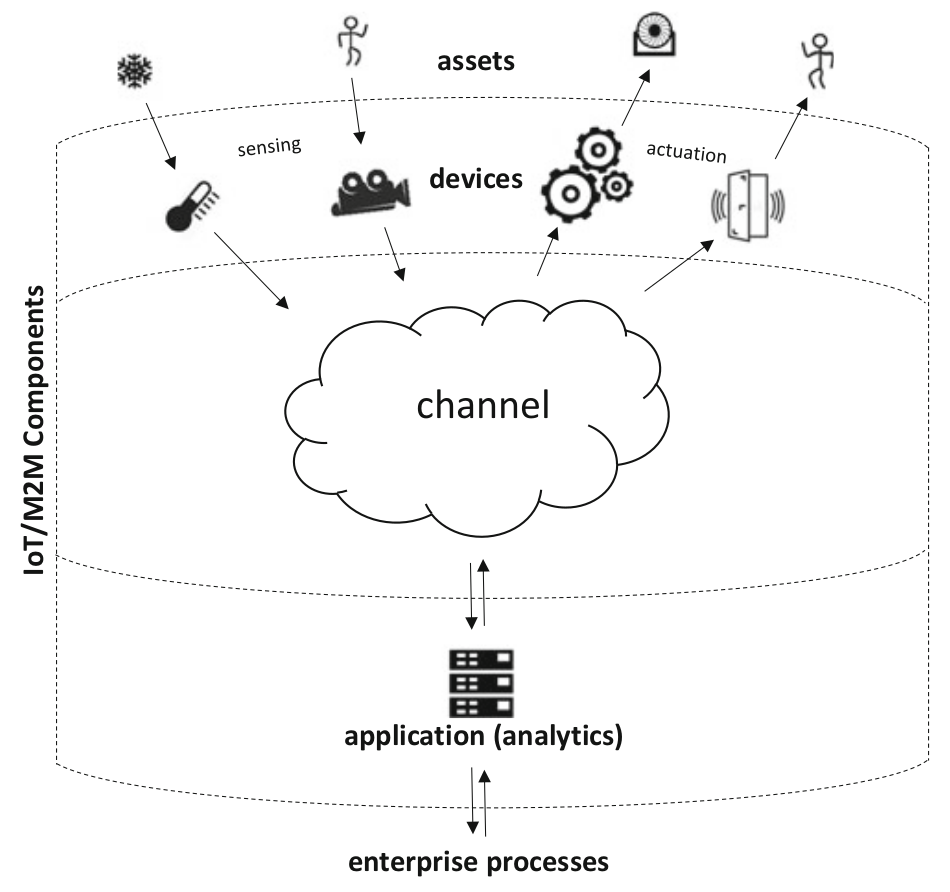
\includegraphics[width=\linewidth]{Pictures/IoT Components.png}}
\caption{M2M/IoT system components}
\label{fig:IoT_components}
\end{figure}


%%%%%  From MTC to IoT  %%%%%%
Most MTC systems are build and designed in vertical nature. This means that they just deal with one type of parameters (i.e. position, speed, humidity, pressure, temperature, etc) and satisfy a very particular application (i.e. turn on/off a switch). The heterogeneous nature of MTC applications lead to a wide range of proprietary networking protocols that serve a single purpose. This lack of standardization has limited the interaction between different applications and slowed down the full automation transition. It was obvious that a horizontal expansion has to be introduced to allow the inter-operation between different applications. Existing for many years and showing its efficiency the Internet Protocol (IP) was the logical candidates to enable this change. An IP-based connectivity framework that links the devices with servers who run the applications is the typical form of today's IoT systems. Figure \ref{fig:M2M_vs_IoT} or \ref{fig:M2M_vs_IoT2} illustrates the main difference between MTC and IoT systems.
\begin{figure}
\centerline{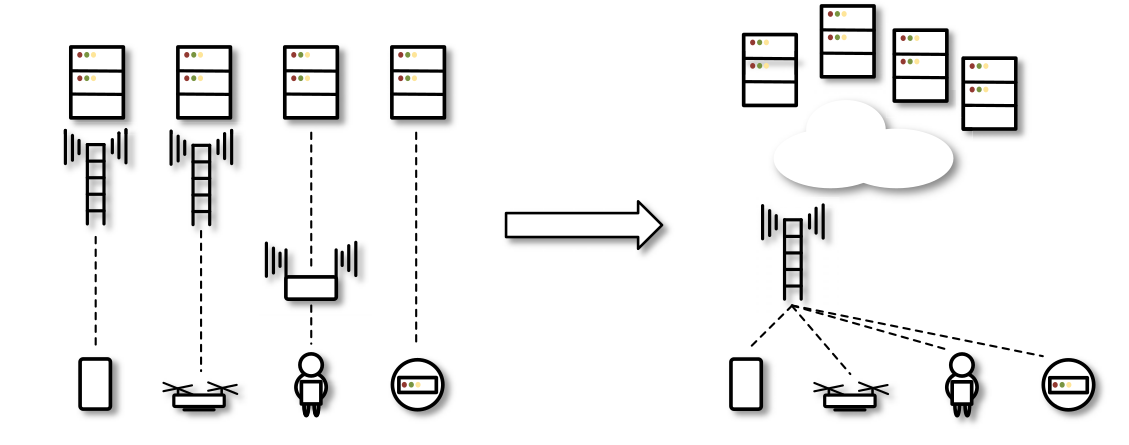
\includegraphics[width=\linewidth]{Pictures/M2M to IoT.png}}
\caption{M2M vs IoT Systems}
\label{fig:M2M_vs_IoT}
\end{figure}

\begin{figure}
\centerline{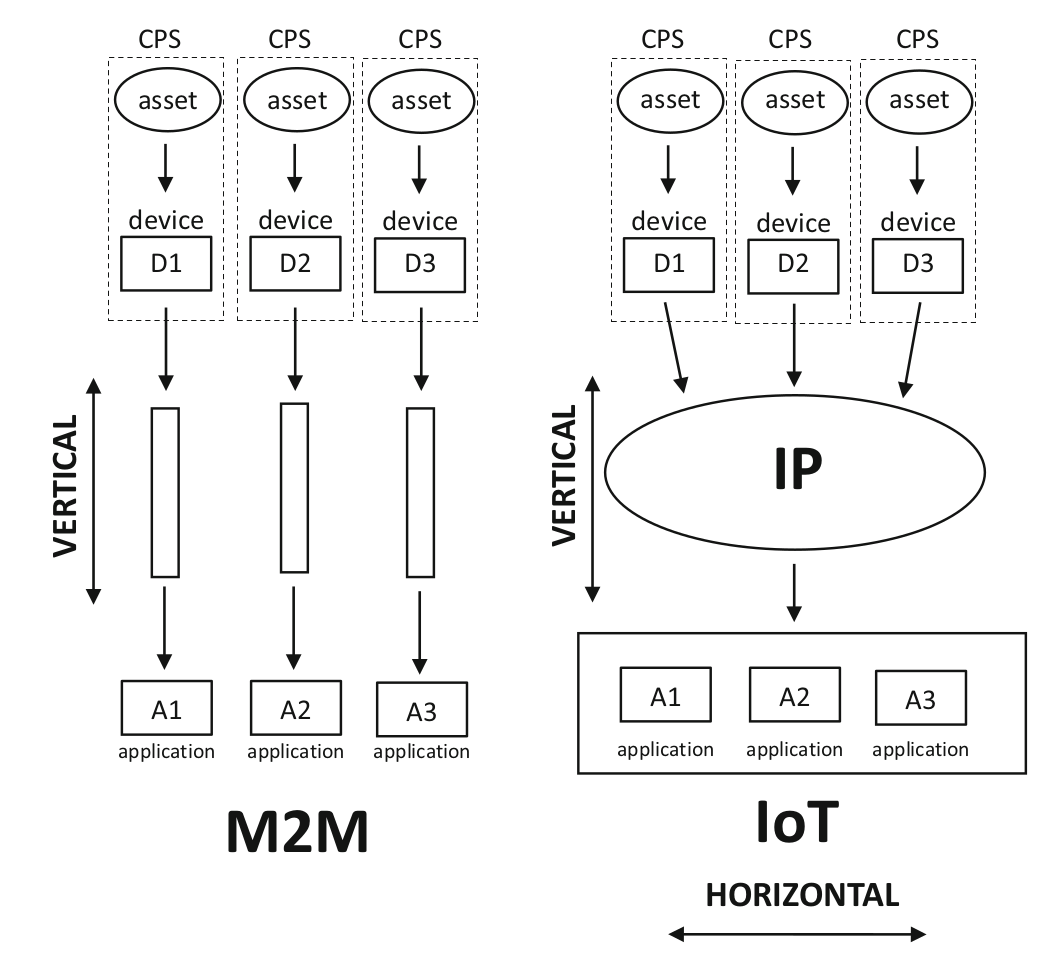
\includegraphics[width=\linewidth]{Pictures/M2M to IoT 2.png}}
\caption{M2M vs IoT Systems 2}
\label{fig:M2M_vs_IoT2}
\end{figure}

%%%%%  What is IoT  %%%%%%
There is no one definition of IoT systems that was agreed on worldwide where every company tries to adopt one that is aligned with its strategy in the market.
%     A network connecting (either wired or wireless) devices, or ‘things’, that is characterized by autonomous
% provisioning, management, and monitoring. The IoT is innately analytical and integrated (IDC)
%     IoT is the next evolution of the Internet, connecting the unconnected people, processes, data, and things in
% your business today (Cisco)
%     IoT devices as those capable of two‐way data transmission (excluding passive sensors and RFID tags). It
% includes connections using multiple communication methods such as cellular, short range and others.
% (GSMA)
%     Sensors & actuators connected by networks to computing systems. These systems can monitor or manage the
% health and actions of connected objects and machines. Connected sensors can also monitor the natural world,
% people, and animal” (McKinsey)
However in 2012, the International Telecommunication Union (ITU) has defined IoT systems in more general way as follow \cite{itu-t_overview_2012_Y.2060}:
\begin{quote}
"A global infrastructure for the information society, enabling advanced services by interconnecting (physical and virtual) things based on existing and evolving inter-operable information and communication technologies (ICT)."
\end{quote}
Things according to ITU can be perceived as \textit{physical} or \textit{virtual} objects that have minimum communication capabilities allowing them to be identified and integrated into information networks. Physical things are equipments of the real world that are usually able to collect, store and process data (e.g., sensors, controllers, and actuators, ...). On the other hand, virtual things are elements of the information word that can stored, processed and accessed such as software applications and multimedia content. It's important to note that the advancement of IoT is based on the foundations of existing and evolving information and telecommunication technologies, including Machine Learning, Cloud Computing, \hl{hardware breakthroughs}.


%%%%%  IoT Networks: Characteristics/Requirements %%%%%%
From a networking prospective, IoT is a network of networks that are connected through some communications and information infrastructure. IoT networks share some defining characteristics that can differ from one use case to another. Here is a list of features that are generally associated to IoT networks \cite{noauthor_y2060_nodate,3gpp_service_nodate_22.368}:
\begin{itemize}
    \item Enormous scale: the number of connected devices in the network that need to be managed is in magnitudes larger than the traditional human-centered communication.
    \item Interconnectivity: in the foreseen vision of IoT, all devices can be interconnected to a global communication infrastructure.
    \item Heterogeneity: Devices in the IoT are based on different hardwares and connected through variable information and communication platforms.
    \item Stochastic nature: The parameters of the network e.g., the number of connected devices, their location and traffic varies in a very dynamic and unpredictable way.
    \item Low-capability devices: In most of IoT application, devices are battery-powered and should autonomously work for several years. This imposes that IoT devices have low processing and storage capacity to minimize power consumption.
    \item Simple design: Since the capabilities of the IoT devices are limited, it is important to have light communication protocol and network architecture.
    \item High-level requirements: some additional functions such as identification, authentication, charging, and security are relevant to the IoT. These requirements can be addressed either using services provided by an intermediary network or using some proprietary solutions.
\end{itemize}.

%%%%%  What is IoT Network architecture? %%%%%%



%%%%%  What is the classification of IoT applications based on requirements? %%%%%%

To better define the requirements that a certain use case puts on the devices and the supporting network, the information and communications technology (ICT) industry leader Ericsson has introduced a novel classification of Cellular IoT in the segments massive IoT, broadband IoT, critical IoT and industrial automation IoT as described in [2] and shown in Fig. 1.5.


IoT application can be classified as in figure \ref{fig:IoT_applications}

\begin{figure}
\centerline{\includegraphics[width=\linewidth]{Pictures/IoT applications.png}}
\caption{IoT applications}
\label{fig:IoT_applications}
\end{figure}


\begin{itemize}
    \item   Massive IoT
    \item   Broadband IoT
    \item   Critical IoT
    \item   Industrial IoT ???
\end{itemize}


%%%%%   What the reader is expected to see in the current article?  %%%%%%
\emph{The goal of this article is to review, analyze and discuss recent developments observed in standardization }



\CAREPL{It is intended to provide updated information for the practitioners and help them 1) select the IoT technology 2) understand what technology will be shortly available}{(write something like this)}



\begin{figure}
\centerline{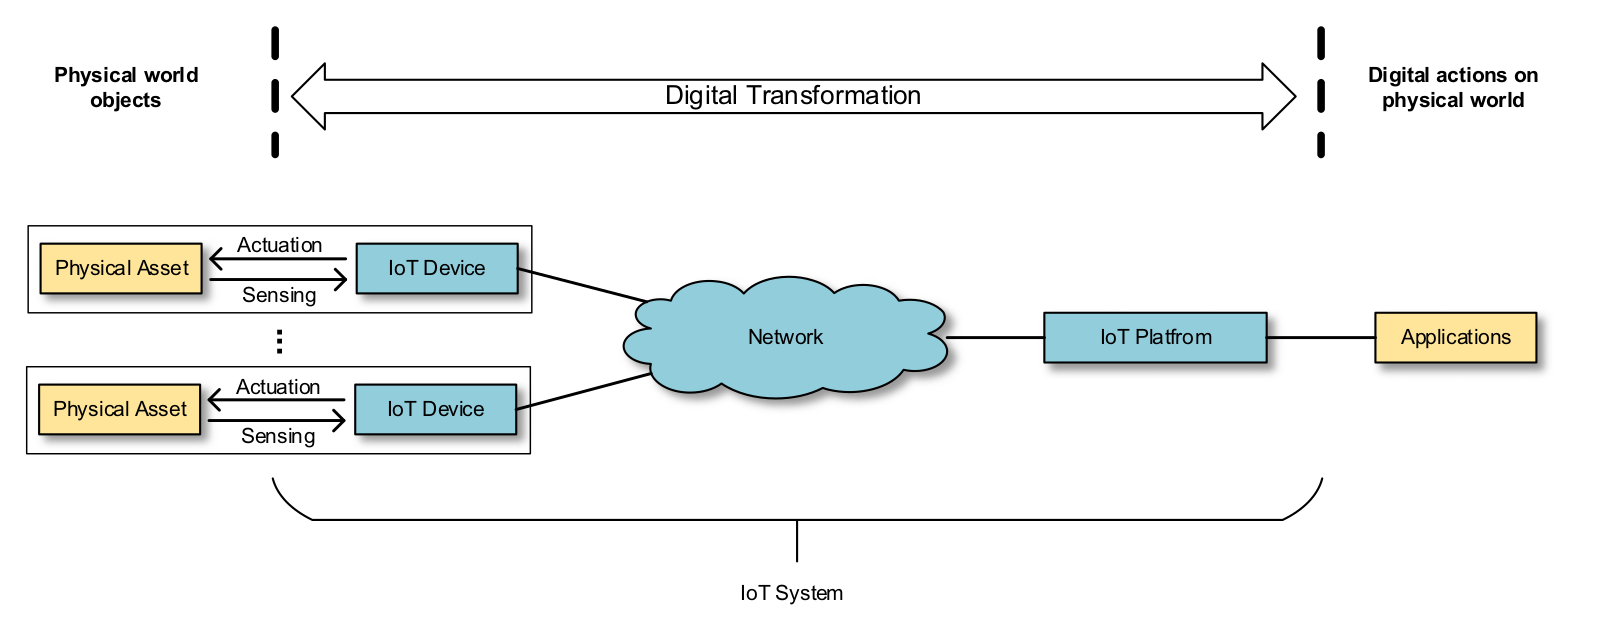
\includegraphics[width=\linewidth]{Pictures/IoT system providing connectivity, services and a digital representation of the physical world.png}}
\caption{IoT system providing connectivity, services and a digital representation of the physical world}`
\label{fig:IoT_sys-ex}
\end{figure}



\section{IoT Connectivity Standards}
\label{sec:2-IoT-Connectivity}


%   Try to Put the best reference that explains each technology and critique them

% This paragraph tries to answer the following questions:
%     -   What are the existing IoT solutions/technologies for IoT Connectivity?
%     -   What is the current deployment in the market of each of these technologies?
%     -   What are the main features of each of them?
%     -   A preamble to the next section? (The emerge of new application and the birth of RedCap in 5G)

It has become clear that the breadth of IoT use cases cannot be described with a simple set of cellular IoT requirements.


This section is meant to summarize all existing telecommunication standards targeting IoT application. See Chapter I in [CIoT textbook] \cite{liberg_cellular_2019} entitled "The Internet of Things"

The evolution of wireless communication has paved the way for the development of IoT 

The IoT connectivity has been a hot topic over the last decade. However, the lack of standardization and the tendency to use single-service solutions have limited the expansion of IoT Networks. The upcoming new fifth generation of mobile network will pave the way for many new IoT use cases and make the transition to the world of smart cities a reality. In order to fully support IoT networks in 5G, a new resource allocation techniques need to be considered to make sure that the introduction of this new service will not affect the other existing service.


Since the IoT services are widely diverse, there is no single connectivity solution that can fit them all. There are several solutions used for IoT connectivity sensors, controllers, and actuators which \emph{(add an example or two about the IoT use cases)}.


The Internet of Things (IoT) starts with connectivity, but since IoT is a widely diverse and multifaceted realm, you certainly cannot find a one-size-fits-all communication solution. Continuing our discussion on mesh and star typologies, in this article we’ll walk through the six most common types of IoT wireless technologies.
\cite{herrero_fundamentals_2021}.
Each solution has its strengths and weaknesses in various network criteria and is therefore best-suited for different IoT use cases.
IoT use cases can be grouped into three main categories. 


\begin{quote}
"Connectivity is the foundation for IoT, and the type of access required depends upon the
nature of the application. Many IoT devices are being served by radio technologies that
operate on unlicensed spectrum and are designed for short-range connectivity with limited
Quality of Service (QoS) and security requirements typically applicable to a home or indoor
environment. Currently, there are two alternative connectivity tracks for IoT applications
that depend on wide-area coverage"

"However, these technologies suffer from some fundamental limitations that limit their wide implementation for
MTC. The main drawback is the lack of efficient backhaul, which limits network scalability and coverage. Another issue is their operation over unlicensed frequency bands, making the communication links unreliable and susceptible to interference. Therefore, it is challenging to support applications requiring a high degree of reliability. Cellular systems, such as Long Term Evolution (LTE), are considered as alternative solutions for the wide provision of MTC applications. Their ubiquitous presence reduces network installation cost and provides widespread coverage and mobility support. In addition, since cellular systems are regulated and interference
controlled, their communication links are more reliable."

\end{quote}

\subsection{3GPP}
\label{sec:1-1}


\begin{quote}


    "
    Since the 80s of last century when the first cellular phone comes into being, the telecommunication industry has experienced four generations development.
    On the one hand, from the initial human-to-human (H2H) communication to the subsequent human-to-machine (H2M) communication, it is intuitive for the researchers to breed the idea of machine-to-machine (M2M) communication. On the other hand, from the business point of view, the volumes of the legacy voice services (represented by H2H) have long since touched the top ceilings; afterwards, the vigorous expansions of the 4G networks have already successfully turned the data services (represented by H2H and H2M) into the master income sources of the mobile operators and promoted them to reach a new revenue summit. Where is the next blue ocean? As far as it goes, the answer seems to
    be the M2M communication, supported by the diverse IoT technologies. This is a tremendous market. By 2020, it is expected that the IoT connections in the world will reach tens of billions level, far exceeding the number of concurrent personal computers and mobile phones [2]; moving forward to 2024, the overall IoT industry is expected to generate a revenue of 4.3 trillion, coming from different sectors, such as device connectivity, manufacturing, and other value added services [3]. To date, IoT is playing an important role in pushing the global economic growth, and is even possible to become the driving force initiating the fourth industrial revolution [4].
    "
    
    
    "
    Cellular IoT is the technology that connects physical objects to the Internet utilising the same cellular network currently used by smartphones. In other words, this technology can connect IoT devices using existing mobile networks. Thus, it eliminates the need to invest and develop a separate dedicated network infrastructure just for IoT devices.
    
    Thanks to significant investments in developing cellular networks in most counties, mobile users enjoy functional cellular connectivity at all times. The idea behind Cellular IoT enablement is to use cellular networks, including 3G, 4G/LTE or 5G, for connecting devices like streetlights, agricultural, and healthcare equipment.
    "

    "
    IoT use cases can be grouped into three main categories. The mobile networks was originally designed to support human to human (H2H) communication. 3GPP addressed the problem of supporting MTC communication since early in release 10 by defining the service requirement for Machine-Type Communications (MTC) in their technical specification 22.368 \cite{3gpp.22.368} . H2H and patterns and requirements of machine to machine (M2M) communication in the IoT are different to those of human to human (H2H) communication in traditional LTE networks. The 3GPP have identified in [4] the following requirements which are specific to M2M communications.
    "
\end{quote}

\textit{Highlight the important role of new wireless telecommunication technology (Cellular or unliscensed) in paving the way for the existence of IoT and MTC in general. In other words, present the advancement in wireless connectivity as the main enabler for IoT. As a complement for this section, we can add a figure showing the wide range of application and the different use cases  use supported. Like the one in by Nokia \ref{fig:iot-use-cases}.}

\begin{figure}
    \centering
    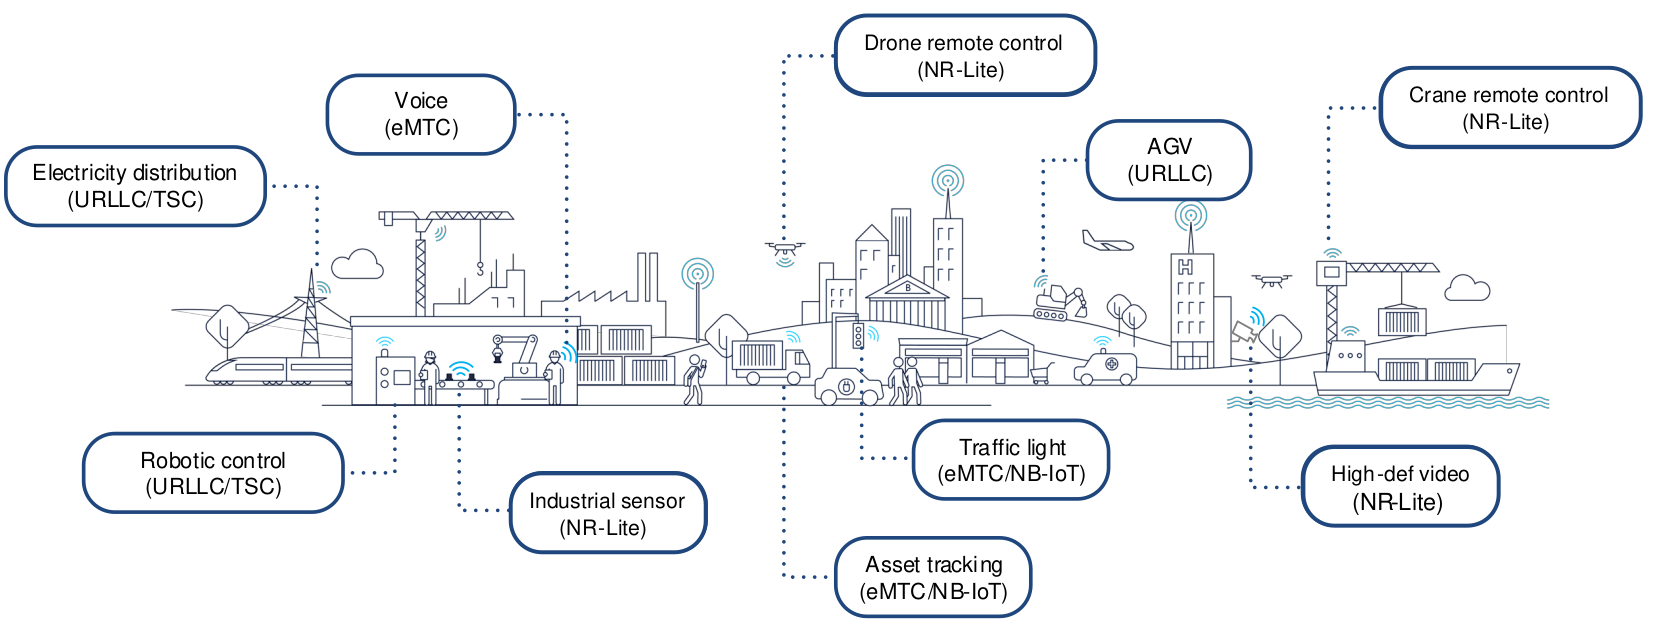
\includegraphics[width=\linewidth]{Pictures/IoT Use Cases.png}
    \caption{IoT use cases}
    \label{fig:iot-use-cases}
\end{figure}


\subsubsection{Narrow-Band IoT}
\label{sec:1-1-1}

Provide similar diagram for RedCap \ref{fig:nb-iot}
\begin{figure}
    \centering
    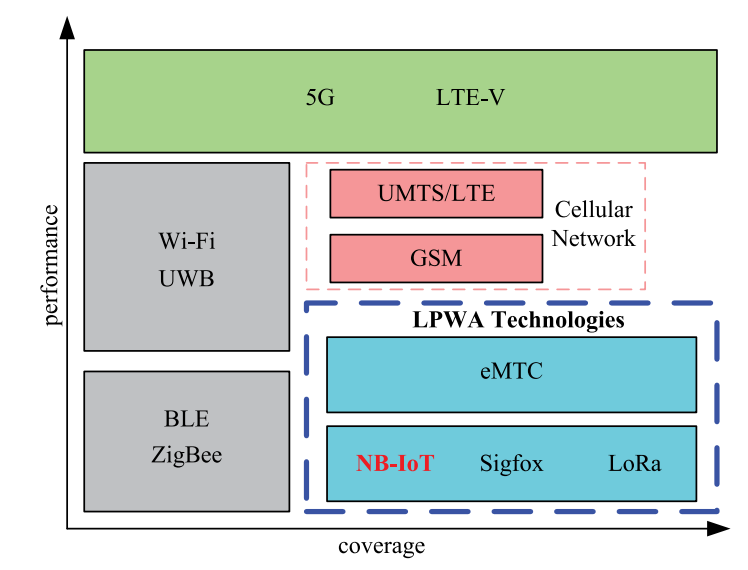
\includegraphics[width=\linewidth]{Pictures/NB-IoT example.png}
    \caption{CIoT standards}
    \label{fig:nb-iot}
\end{figure}

\subsubsection{LTE-M}
\label{sec:1-1-2}

\subsubsection{EC-GSM}
\label{sec:1-1-3}

Compare IoT technologies in 3GPP \ref{fig:3gpp_ciot}
\begin{figure}
    \centering
    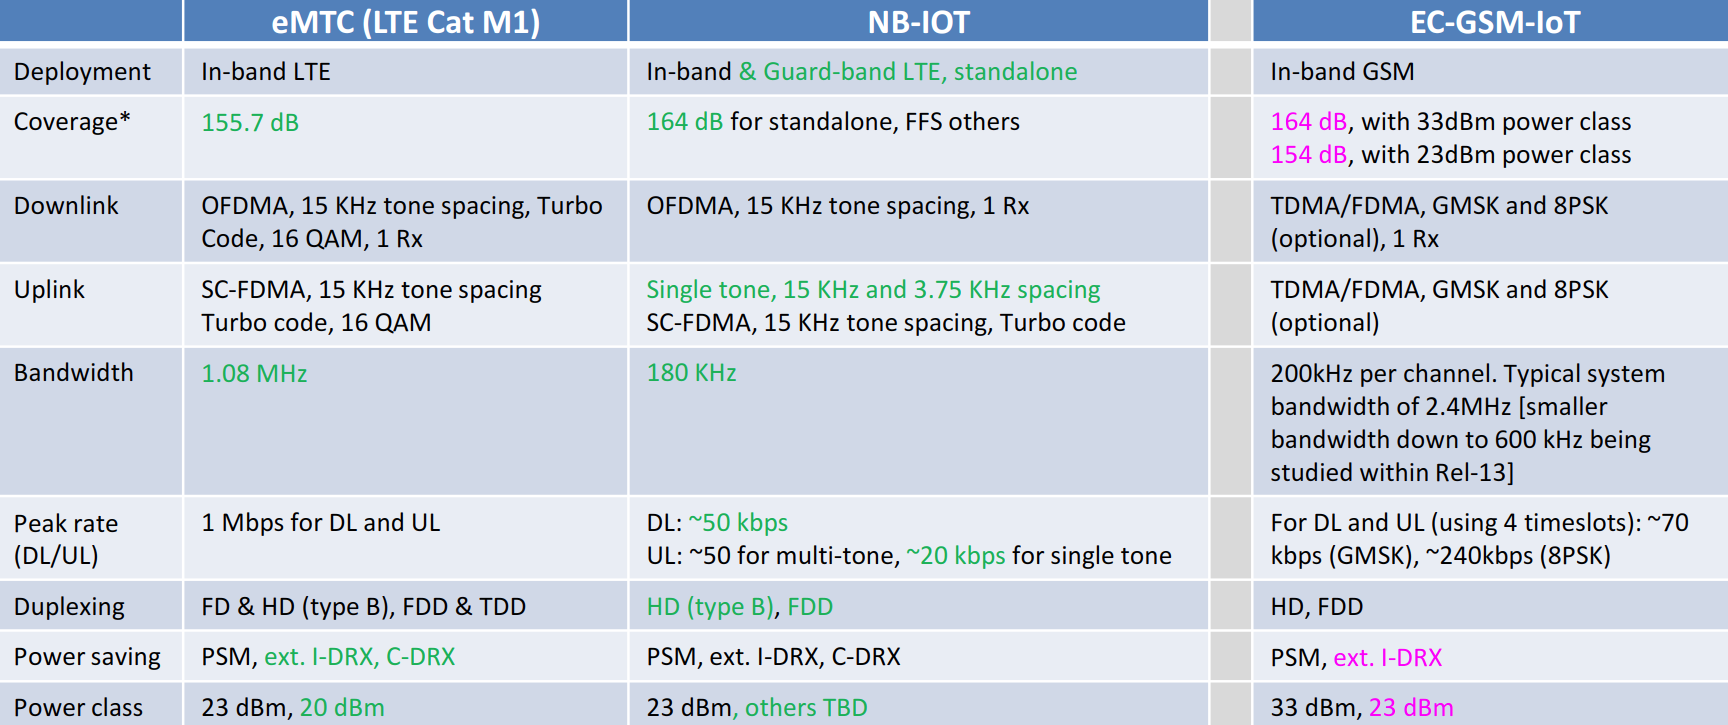
\includegraphics[width=\linewidth]{Pictures/3GPP CIoT.png}
    \caption{CIoT standards}
    \label{fig:3gpp_ciot}
\end{figure}

\subsection{Unlicensed}
\label{sec:1-2}

\subsubsection{LoRa}
\label{sec:1-2-1}
LoRa, stands for Long Range. It is a physical layer
LPWAN solution that modulates signals using a spread
spectrum technique designed and patented by Semtech
Corporation [11]. Technically, LoRa employs the chirp spread spectrum (CSS) modulation that spreads a narrow-
band signal over a wider channel bandwidth, thus en-
abling high interference resilience and also reducing the
signal-to-noise-and-interference ratio (SINR) required at
a receiver for correct data decoding [106]. The spreading
factor of the CSS can be varied from 7 to 12, which makes
it possible to provide variable data rates and tradeoff
between throughput and coverage range, link robustness,
or energy consumption [20], [23]. Specifically, a larger
spreading factor allows a longer transmission range but at
the expense of lower data rate, and vice versa. Depending
on the spreading factor and channel bandwidth, the data
rate of LoRa can vary between 50bps and 300kbps.
In 2015, a LoRa-based communication protocol called
LoRaWAN was standardized by LoRa-Alliance [107].
LoRaWAN is organized in a star-of-stars topology, where
gateway devices relay messages between end-devices and
a central network server [25]. In LoRaWAN, three types
of devices (Class A, B, and C) with different capabilities
are defined [108]. In particular, Class A is the class of
LoRaWAN devices with the lowest power consumption
that only require short downlink communication, and
Class A devices use pure-ALOHA RA (please refer
to Appendix A for more details and explanations on
ALOHA protocols) for the uplink. Class B devices are de-
signed for applications with extra downlink transmission
demands. In contrast, Class C devices have continuously
receive slots, thus always listening to the channel except
when they need to transmit. Among the three classes, all
the devices must be compatible with Class A [25].
\subsubsection{sigfox}
\label{sec:1-2-2}
SigFox is another dominant unlicensed LPWAN
solution on the market [10]. SigFox proposes to use an
ultra narrow-band (UNB) technology with only 100Hz
bandwidth for very short-payload transmission. Thanks to
the UNB technology, Sigfox enables less power consump-
tion for devices and supports a wider coverage compared
with LoRA at the cost of a lower data rate [110]. Sigfox
was initially introduced to support only uplink communi-
cation, but later it evolved to a bidirectional technology
with a significant link asymmetry [111]. However, the
downlink transmission can only be triggered following
an uplink transmission. In addition, the uplink message
number is constrained to 140 per day and the maximum
payload length for each uplink message is limited to
12bytes [23]. Due to these inflexible restrictions, together
with its unopened business network model [20], Sigfox
has unfortunately shifted the interest of academia and
industry to its competitor LoRaWAN, which is considered
more flexible and open. In Table IV, the characteristics
of Sigfox and LoRa are summarized.
Compare all available IoT technologies fig\ref{fig:all-iot}




\begin{figure}
    \centering
    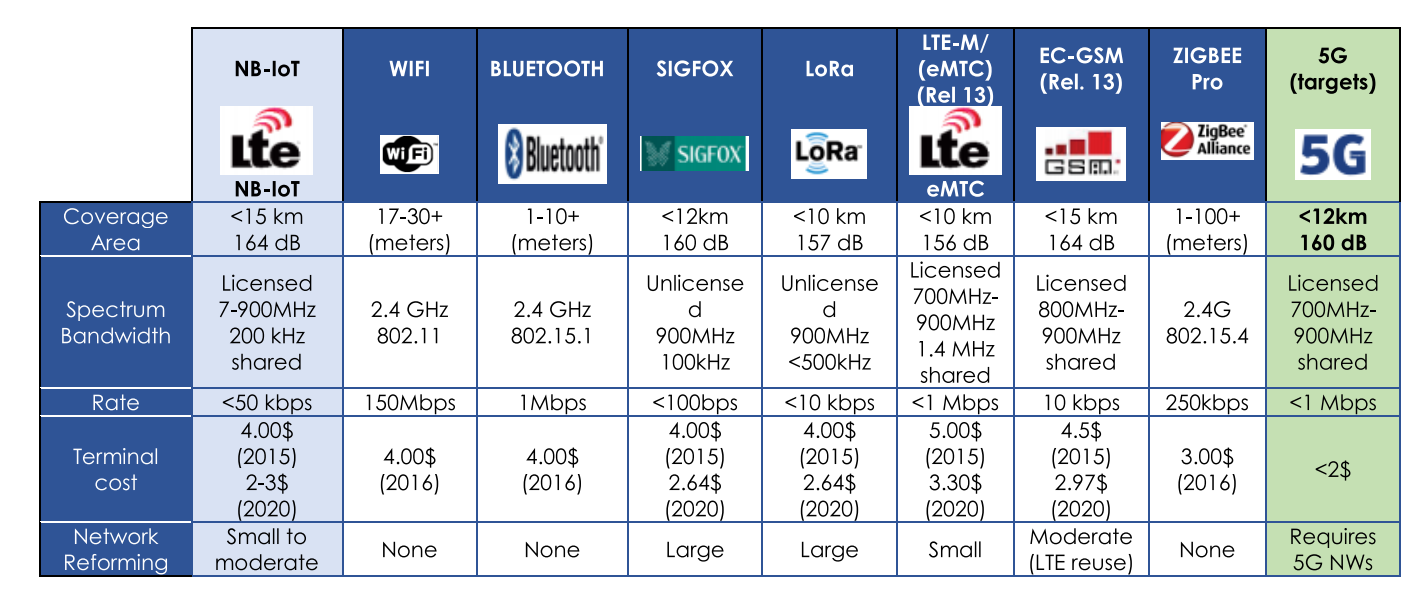
\includegraphics[width=\linewidth]{Pictures/IoT standards.png}
    \caption{CIoT standards}
    \label{fig:all-iot}
\end{figure}



\section{Reduced Capability Devices}
\label{sec:3-RedCap-Intro}

% This paragraph tries to answer the following questions:
%     -   What is the current state of 5G? (Existing usage scenarios)
%     -   What are the new market sectors in IoT available for 5G?
%     -   Why we need a new category to support these new use-cases? (Justification)
%     -   What is the definition of RedCap?
%     -   What are the requirements of RedCap devices?
%     -   What is the standardization process?
%     -   Preamble to the next section?


%%%%%   The Main classes of 5G before Rel-17  %%%%%% Good
The early 5G system in Rel-15/16 was originally intended to support three main usage scenarios, namely, enhanced mobile broadband (eMBB), ultra-reliable and low-latency communications (URLLC), and massive machine type communications (mMTC). These three classes have significantly heterogeneous requirements in terms of data rate, latency, connection density, energy efficiency, reliability, and mobility. ITU has identified the minimum technical performance requirements for 5G services known as the IMT-2020 standard. These features have been summarized in the report M.2410-0 \cite{itu-r_minimum_2017_M.2410-0}.

%%%%%   URLLC and mMTC  %%%%%%
 Both URLLC and mMTC are intended to target novel IoT use cases. URLLC features, which are supposed to target time-sensitive applications, were primarily introduced in Rel-15. A further enhanced version was introduced in Rel-16 within the enhanced URLLC (eURLLC) work item \cite{3gpp_study_nodate_38.824}.

%%%%%   Smart factory and vertical industries  %%%%%%
One of the important goals of 5G systems is to enable the automotive industry. The framework of Industry 4.0 aims to create more interconnected smart factories. This industrial transformation can help improve efficiency, reduce operational costs, increase safety, and enhance productivity. All these efforts play an important role almost in all vertical industries, including logistics, healthcare, manufacturing, transport, construction, and power grid. It is important to note that developing massive industrial wireless sensor network is the base to achieve this hoped transformation. 

%%%%%   Smart cities  %%%%%%
Similar to smart factories, 5G is vital in the new transformation toward smart cities. The smart city verticals include a variety of city activities such as lighting, transport, waste, parking, video surveillance, etc. The collected data can help in efficiently managing and controlling city resources and improve services provided to residents.

%%%%%   Wearables  %%%%%%
Another important component of 5G future smart community is Wearables. Devices like smartwatches, extended reality (XR) devices, and medical devices will have a huge impact on everybody's life.

%%%%%   New mid-IoT fall in Between %%%%%%
These mid-range use-cases have requirements that fall in-between those of eMBB, URLLC, and mMTC. They are demanding a performance higher than what is offered by mMT but lower than URLLC and eMBB as shown in figure \ref{fig:redcap-spider} from M.2410-0. 
\begin{figure}
    \centering
    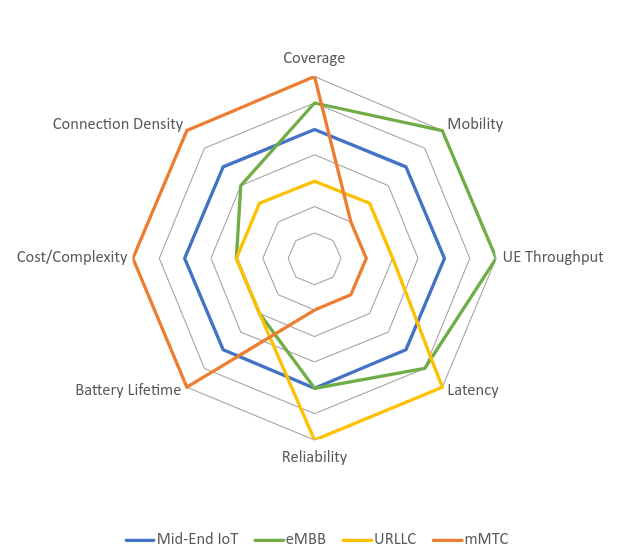
\includegraphics[width=\linewidth]{Pictures/Radar Chart RedCap.png}
    \label{fig:redcap-spider}
    \caption{RedCap Radar chart}
\end{figure}

%%%%%   The need for new class in 5G  %%%%%%
Therefore it is important to further optimize the network resources and more efficiently support such mid-range IoT applications. In this regard, 3GPP has initiated in Rel-17 the work to support a new category of devices with a reduced cost/complexity compared to the high-end Rel-16 eMBB and URLLC NR devices. This new category of devices was presented as a light-weight version of NR devices under the name NR-Light or NR-lite. Now it is officially called Reduced Capability devices (RedCap).

%%%%%   The introduction of RedCap  %%%%%%
The main objective of this UE new category to serve three reference use cases: Industrial wireless sensors (e.g., various kinds of sensors and actuators), Video Surveillance (e.g., surveillance cameras that are essential for smart city and industries), Wearables (e.g., AR/VR devices, Human-assistive devices, smart watches, glasses,  etc.).

%%%%%   The requirements of RedCap  %%%%%%
Table \ref{table:redcap-requirements} presents the main requirements specified by 3GPP study item on support of reduced capability NR devices TR 38.875 \cite{3gpp.38.875}. From table \ref{table:redcap-requirements} it is noted that these three representative use cases have slightly different requirement. However, they can be categorized in one class of mid-end IoT services to avoid fragmenting the market (R2-2009618\cite{3gpp_framework_2020_R2-2009618}). RedCap devices share a common a generic constraints of being low cost/complexity and compact in size. RedCap devices are also meant to support 5G frequency bands in both frequency range 1 (FR1), and frequency range 2 (FR2), and support the two modes of operation: frequency division duplex (FDD) and time division duplex (TDD).

\begin{table*}
\centering
\caption{Redcap reference use cases and requirements}
\begin{tabular}{|c | c | c | c|} 
 \hline
 \textbf{Requirement} & \textbf{Industrial wireless sensors} & \textbf{Video Surveillance} & \textbf{Wearables} \\ 
 \hline
 Data Rate & \multirow{2}{*} {2 Mbps} & \multirow{2}{*} {7.5-25 Mbps} & 5-50 Mbps in DL (peak 150 Mbps)\\ 
  & & & 2-5 Mbps in UL (peak 50 Mbps) \\
  \hline
 Latency & 100 ms (5-10 ms in safety applications) & 500 ms & - \\
  \hline
 Availability & $99.99\%$ & $99\%-99.9\%$ & - \\
  \hline
 Battery lifetime & few years & - &  Multiple days (up to 1-2 weeks) \\
  \hline
 Traffic pattern & Heavy UL & High-end video (Heavy UL) & - \\ 
 \hline
 Mobility & Stationary & Stationary & Low-Mobility \\
  \hline
Coverage & \multicolumn{3}{c|}{$MCL=143dB$}\\
 \hline
 Cost/Complexity & \multicolumn{3}{c|}{Low cost/complexity devices compared to eMBB and URLLC}\\
 \hline
 Size & \multicolumn{3}{c|}{a design with compact form factor}\\
 \hline
\end{tabular}
\label{table:redcap-requirements}
\end{table*}

%%%%%   Seprate RedCap from other 3GPP   %%%%%%
It is worth mentioning that RedCap devices approximately provide a performance similar to low-end LTE UEs such as Cat-1. Nevertheless, it was agreed to develop RedCap as a 5G standalone technology to benefit from the efficiency of the 5G core network and facilitate the transition to full 5G network. Also, it is important to note that RedCap is not designed to serve low-power wide-area (LPWA) use cases. 3GPP confirmed in its study on "self-evaluation towards IMT-2020 submission" \cite{3gpp_study_nodate-1_37.910} that together LTE-M and NB-IoT fulfill IMT-2020 requirements for mMTC class and they will be considered as 3GPP technologies for LPWA application. Therefore RedCap design reuses NR features in the best way suited for its use cases.

%%%%%   Standarization process and preamble for next sub-section   %%%%%%
In Rel-17 The study phase on the support of RedCap devices was initiated by multiple RAN work groups. The study aimed to find technical solutions to support the new mid-end IoT use cases while having marginal impact on the existing network. It has three main directions/objectives: UE complexity Reduction, UE battery lifetime enhancement, and coexistence with other technologies. The following sections explain in-detail the proposed features and their impact on the performance. The findings of this study item are documented in the technical report TR 38.875 \cite{3gpp.38.875}.The study phase was followed by a work item phase to specify the necessary updates of NR standard, specifically,  UE capabilities (38.306 \cite{3gpp_nr_nodate-4_38.306})  and RRC parameters (38.331 \cite{3gpp_nr_nodate-3_38.331})(see section 4.2.21).

\section{UE complexity reduction}
\label{sec:4-complexity-reduction}

% Note: Give more details on how the gain in cost is achived (Small paragraph saying that each part has a certain gain and the overall gain is an accmulation)



% This paragraph tries to answer the following questions:
%     -   What are the proposed features/enhancement in Rel-17 to reduce the complexity in RedCap devices? For each of these features we state:
%         -   Description
%         -   Gain in terms of cost/complexity
%         -   Potential impact on network performance


%%%%%   Emphasize that RedCap is an extension of NR UE   %%%%%%
The design of low cost/complex devices was the main priority of the RedCap study phase. It is important to note that RedCap devices are built on the foundation of reference Rel-15/16 NR devices. This means that RedCap will try to optimize NR configurations in a way that suits the overseen use cases.

%%%%%   preamble to next subsections   %%%%%%
Many technical solutions have been suggested to reduce UE cost/complexity. Most of these modifications are related to features in the physical layer (e.g., Bandwidth, no. of antennas, etc). In the following we present the main complexity reduction features that were standardized in RedCap Rel-17 \cite{3gpp.38.875}.






\subsection{Reduced number of UE Rx antennas}
\label{sec:4-1}

%%%%%   Feature description   %%%%%%
The support of multi-input multi-output communication is essential for most of  modern day wireless systems. Increasing the number of receiving antennas (Rx) allows, based on the applied signal processing, to dramatically enhance the experienced coverage and throughput at user terminal. However, this desired advantages come at the cost of unpleasant complex RF chains and overhead processing. The reference NR device has to support the following antenna configuration:
\begin{itemize}
    \item In FR1: 2 Rx for FDD mode and 4 Rx for TDD mode
    \item In FR2: 2 Rx
\end{itemize}
While for RedCap UEs 1 Rx and, optionally, 2 Rx configuration were considered in the study.
%%%%%   The improvement   %%%%%%
Reducing the number of Rx branches simplifies both UE RF components (including Antenna array, Filters, LNAs, mixer, and local oscillator) and Base-Band operations (ADC/DAC, FFT/IFFT, Synchronization/cell search block, MIMO processing). The overall device cost/complexity can reach $30-50\%$. More information about the evaluation mythology and the estimation of cost reduction can be found here R1-2009293 \cite{3gpp.R1-2009293}
%%%%%   Negative possible impact   %%%%%%
This cut in the device cost/complexity comes at the expense of degrading network performance. Having one Rx branch limits RedCap devices from performing of MIMO operations and benefiting from spatial diversity. The impacted properties are coverage and spectral efficiency. Nevertheless, RedCap requirements still met. Another aspect concerning the energy consumption, where in-theory it should be reduced due to the usage of fewer Rx branches. However, the time needed to receive a certain payload is increased as result of the small data rate of RedCap devices.

\subsection{UE bandwidth Reduction}
\label{sec:4-2}

%%%%%   Feature description in legacy NR   %%%%%%
Legacy NR devices must support two ranges of carrier frequencies, namely, FR1 and FR1. Within these two possible ranges UE will transmit/receive signals over a carrier bandwidth. In 5G NR, The maximum carrier bandwidth is 100 MHz in FR1 and 200 MHz (optionally 400 MHz) in FR2 (see TS 38.101-1 \cite{3gpp_nr_nodate-2_38.101-1} and TS 38.101-2 \cite{3gpp.38.101-2}). Higher carrier bandwidth can be reached using Carrier Aggregation (CA).
%%%%%   What is done in RedCap   %%%%%%
Given the less demanding requirement of RedCap use cases in terms of data rate, it is possible to decrease the maximum supported bandwidth. For RedCap UEs, the max allowed bandwidth is 20 MHz in  FR1 and 50 MHz (optionally 100 MHz) in FR2. It also abandoned the support of CA for RedCap device.
%%%%%   The gain   %%%%%%
This reduction results in a substantial decrease of device cost/complexity, estimated to be on the order of $\sim30\%$ in FR1 and $\sim20\%$ in  FR2. Most of the registered gain is asocciated with less processing in base-band parts (ADC/DAC, LDPC decoding, ...).
%%%%%   Negative possible impact   %%%%%%
It must noted that this cut has a minor impact on coverage, spectral efficiency, and latency. The main affected metric is the achievable peak data rate. However, it is enough to meet the predefined requirements of RedCap use cases.

\subsection{Half-duplex FDD Operation}
\label{sec:4-3}


%%%%%   Feature description in legacy NR   %%%%%%
One of the main aspects of 5G UE capabilities is the support of duplex communication, i.e., communicate in both direction uplink and downlink. It exists two systems of duplexing: Frequency Division Duplex (FDD), and Time Division Duplex (TDD) [as illustrated in the figure \ref{fig:5g-duplexing}]. FDD implies that DL and DL transmission occurs on different carrier frequencies. On the other hand, in TDD, the separation between the two flow take place in time domain. 
 While FDD offers better coverage due to frequency separation, TDD provides higher throughput because of the simplified processing. In general, a reference 5G device supports both TDD and FDD modes.
 
 Full-Duplex FDD means that the transmission on both DL and UL happens at the same time. On the contrary, Half-Duplex FDD operation obligates that UE is only allowed to receive or transmit at a given time.  This approach of communication gained a lot of attention in LTE for use cases that do not require high throughput but have some constrain on energy consumption such as IoT application. In TS 36.211 \cite{3gpp_nr_2022-2_38.211}, two types of Half-Duplex FDD were defined for Half-Duplex FDD operation: Type A and Type B. The main difference between the two types is the guard period between receiving and transmitting, where Type B allows a wider guard.
\begin{figure}
    \centering
    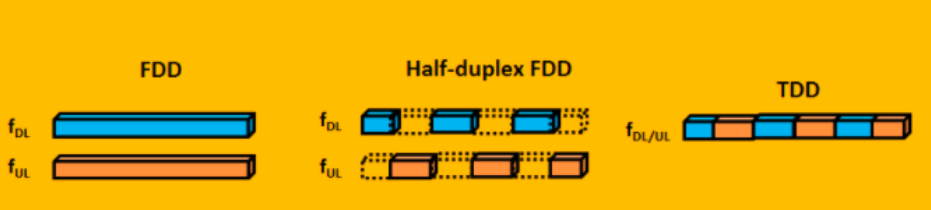
\includegraphics[width=\linewidth]{Pictures/5G Duplexing.png}
    \label{fig:5g-duplexing}
    \caption{5G Duplexing}
\end{figure}

%%%%%   What is done in RedCap   %%%%%%
In the study phase it was suggested to use both types of half-duplex operation  for RedCap devices, where Type A is prioritized.
%%%%%   The gain   %%%%%%
Comparing to a reference NR device having a HD-FDD only device can save  $\sim7\%$ for Type A and $\sim10\%$ for type B. Most of the cost saving comes from replacing the duplexer by a switch and a lowpass filter and having simplified RF transceiver.
%%%%%   Negative possible impact   %%%%%%
However, operating in half-duplex mode may have a negative impact on the latency. Some additional delay can be experienced especially in case of simultaneous DL and UL traffic. Nevertheless, the latency requirement for RedCap use cases is still fulfilled. Also, it worth noting that introducing HD-FDD operation will have some impact on the specification, e.g., UL/DL switching time, applicable bands, etc. 


\subsection{Relaxed maximum number of MIMO layers}
\label{sec:4-4}

%%%%%   Feature description in legacy NR   %%%%%%
One way of using the multiple antennas in wireless systems is spatial multiplexing. Spatial multiplexing based on dividing the transmitted data into several traffic flows (MIMO layers) and send them simultaneously on different available antennas. This very powerful technique helps enhancing the system spectral efficiency and multiplying the achievable data rate.
The reference NR device can support, depending on antenna configuration, up to 4 layers in FR1 and 2 layers in FR2 (\textcolor{red}{See the max antenna configuration and subsequently MIMO layers}). 
%%%%%   What is done in RedCap   %%%%%%
For RedCap the maximum number of MIMO layers was reduced to one layer FR1/FR2 and optionally 2 layer for FR1 TDD.

%%%%%   The gain   %%%%%%
Reducing the maximum number of MIMO layers helps in simplifying the signal processing and eventually the over all cost/complexity. The gain in cost is $\sim17\%$ when reducing from 4 to 1 layers in FR1 TDD and $\sim11\%$ when reducing to 1 layer for the case of FR2
%%%%%   Negative possible impact   %%%%%%
The main impact of cutting the number of supported MIMO layers is decreasing the spectral efficiency and subsequently the achievable data rate. Depending on the situation, the peak rate will decrease by $50-75\%$. Instead of this reduction, RedCap devices can still be able to fulfill defined requirements.

\subsection{Relaxed maximum modulation order}
\label{sec:4-5}

%%%%%   Feature description in legacy NR   %%%%%%
Modulation order is an important factor that affect the experienced throughput. Having a higher modulation order can dramatically increases the spectral efficiency (e.g, 256QAM=8 bits per symbol).

%%%%%   What is done in RedCap   %%%%%%
In RedCap study and in order to cut the device cost, it was suggested to change maximum mandatory modulation orders for RedCap as follow: 64QAM instead of 256QAM for the DL  and 16QAM instead of 64QAM for UL.

%%%%%   The gain   %%%%%%
The proposed relaxation of modulation orders decrease the device cost/complexity by reducing the required processing in both RF and base-band. The estimated reduction in the cost is $\sim6\%$ for downlink case and $\sim2\%$ for the uplink

%%%%%   Negative possible impact   %%%%%%
Similar to the reduction of maximum MIMO layers the main impacted parameter here is the spectral efficiency and subsequently the achievable data rate. The peak rate will decrease by $25-33\%$, depending on the considered relaxation. 

\subsection{Combinations of UE complexity reduction features}
\label{sec:4-6}
In addition to the techniques listed in subsections A-E, other features related to higher layers were discussed in the study phase of RedCap. This includes, Reduction of maximum number of data radio
bearers (DRBs), Reduction of sequence number (SN) in PDCP and RLC, Reduction of L2 buffer size, etc. However, they were not part of the final recommendations for the design of RedCap devices because they needed additional changes to the specification and their incorporation in reducing the device cost was marginal.

Alongside studying individual techniques, it was suggested to mix some of them together. Different combination of complexity reduction features and their impact on the the device overall material cost are presented in TR 38.875 (See Table 7.8.2-1, Table 7.8.2-2, and Table 7.8.2-3). Cost decrease in the order of $50-70\%$ was gained. For example, using the following setting of 20 MHz, 1 layer, 1 Rx, DL 64QAM, and UL 16QAM together instead of the reference NR device in FR1 TDD can achieve an estimated cost reduction of $\sim70.7\%$.

At the end of this section we summarize in table \ref{table:redcap-features} the list of recommendations published by 3GPP for designing RedCap devices. It is important to note that these techniques does not require a dramatic change in the specification of 5G NR nor deteriorate the network performance. \textcolor{red}{However}, they can bring a substantial reduction in cost, complexity, and size of user terminal. In the following section a review of the possible methods proposed to enhance UE battery lifetime, which was the second objective of RedCap.
\begin{table*}
\centering
\caption{RedCap main features}
\begin{tabular}{|c | c | c | c| c|} 
 \hline
    & \multicolumn{2}{c}{\textbf{FR1}}  &  \multicolumn{2}{c|}{\textbf{FR2}} \\
  \cline {2-5}  
    & Ref. NR device & RedCap device & Ref. NR device &  RedCap device\\
\hline
 Bandwidth      & 100 MHz & 20 MHz  & 200 MHz  &  100 MHz \\
\hline
\multirow{2}{*} {Min number of Rx branches} & FDD: 2 Rx & \multirow{2}{*}{ 1 or 2 Rx }& \multirow{2}{*}{ 2 Rx } &  \multirow{2}{*}{ 1 or 2 Rx }  \\
& TDD: 4 Rx & &   &   \\
\hline
Duplexing Mode   & FDD and TDD &  Half-duplex FDD & TDD &  Half-duplex FDD \\
\hline
 \multirow{2}{*} {Max modulation order} & DL: 256QAM & DL: 64QAM  & DL: 64QAM  &  DL: 16QAM \\
& UL: 64QAM  & UL: 16QAM  & UL: 64QAM  &  UL: 16QAM \\
\hline
 Max MIMO Layers   & 4 or 2 & 1 or 2  & 2   &  1 or 2 \\
\hline
 Cost Reduction   & 0$\%$ & 70$\%$  & 0$\%$  &  50$\%$ \\
\hline
\end{tabular}
\label{table:redcap-features}
\end{table*}

\section{UE power-saving enhancement}
\label{sec:5-power-saving}

% Note: Give more details on how the gain in cost is achived (Small paragraph saying that each part has a certain gain and the overall gain is an accmulation)


% This paragraph tries to answer the following questions:
%     -   What are the enhancement related to UE power-saving proposed in SI TR 38.84? 
%     -   What are the additional enhancement available for RedCap devices? For each of these features we state:
%         -   Description
%         -   Gain in terms of cost/complexity
%         -   Potential impact on network performance



%%%%%   The importance of Power Saving and the work of 3GPP   %%%%%%
Another important objective of the work on reduced capability devices is to enhance the UE device energy consumption and extend the battery lifetime of the UE. In fact, enhancing UE power-saving is one of the main goals of 5G Rel-16, where a study item TR 38.840 \cite{3gpp.38.840} entitled "Study on UE power saving in NR" was created. This study item suggested multiple technical solutions that can be adopted by the UE to more efficiently consume energy. All the added features related to power-saving will be available by default for RedCap devices

%%%%%   Power Saving for RedCap   %%%%%%
Beyond that, given the low-mobility/stationary nature of the RedCap device along with the bursty intermittent traffic, additional enhancement were proposed to further improve UE power-saving . The three main features were discussed in the RedCap study pahse:
\begin{enumerate*}
    \item Decrease the number of blind decodes of PDCCH channel,
    \item Extend sleep time of discontinuous reception (DRX) in Idle/Inactivity states
    \item and the Relaxation of RRM measurements. 
\end{enumerate*}
However, only the last two were included later in the work item of RedCap Rel-17 \cite{3gpp_revised_2022-1_RP-220966}, the first feature was abandoned due to the marginal enhancement it adds to power consumption $0-12\%$ and its big impact on PDCCH blocking rate and consequently the latency \cite{ratasuk_reduced_2021}. The following subsections present in more details the description of the two proposed power-saving features and their potential improvement.

\subsection{Extended DRX for RRC Inactive/Idle}
\label{sec:5-1}

%%%%%   UE listen to PDCCH for DCI   %%%%%% (Resource Grid for Corset, DCI formats,)
In 5G system, gNBs transmits messages of Downlink Control Information (DCI) over the physical downlink control channel (PDCCH). These DCI messages have multiple formats based on the information they want to convey to UE  e.g, allocated time/frequency resources on the uplink and downlink, UL power-control, etc. UEs monitors several PDCCHs, typically one per slot TR 21.915 \cite{3gpp.21.915}. However, for some low latency applications (e.g., URLLC) UEs can be configured to monitor PDCCH more frequently. Upon detection of valid PDCCH, UE follows the control information contained in DCI message.

%%%%%   Description of the concept of discontinuous reception   %%%%%%
In fact, most of the time UE does not have any data to send/receive and this continuous monitoring of PDCCH messages can lead to unnecessary excessive energy consumption. To solve this problem, in 5G NR, UEs are allowed to discontinuously monitor the PDCCH and turn off their transceiver chains achieving more power-saving. In fact, Discontinuous Reception (DRX) is considered one of the main power-saving measures that has been adopted by many 3GPP cellular technologies before 5G. When UE has a DRX option configured it will periodically alternate between active (ON) and sleep (OFF) periods in a duty cycle scheme as shown on the figure \ref{fig:5g-drx}. Depending on the state of the UE, i.e., RRC\_CONNECTED, RRC\_idle/inactive, there exist two modes of DRX: Connected mode DRX (CDRX) idle/inactive mode DRX (IDRX).

\begin{figure}
    \centering
    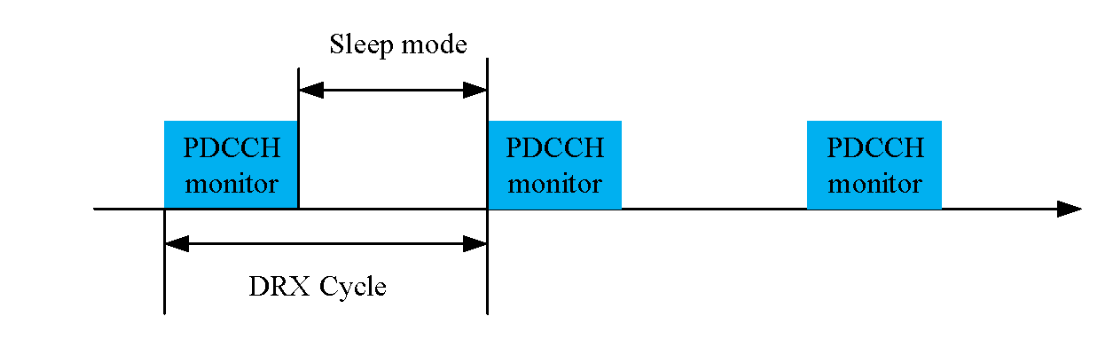
\includegraphics[width=\linewidth]{Pictures/Schematic diagram of DRX.png}
    \label{fig:5g-drx}
    \caption{Schematic diagram of DRX}
\end{figure}


%%%%%   CDRX in detail %%%%%%
    In CDRX, the Radio Resource Control (RRC) entity controls DRX operation by configuring the following parameters (see TS 38.331 \cite{3gpp_nr_nodate-3_38.331}) in the Media Access Control (MAC) layer:

\begin{itemize}
    \item \textit{drx-LongCycleStartOffset}: configure two parameters \textit{drx-LongCycle} and \textit{drx-StartOffset}. The first one sets the duration of DRX cycle and has the values between 10 ms and 10.24 s. On the other hand, drx-StartOffset defines the starting point for the ON duration and has the value in multiples of 1 ms (see the illustration on figure \ref{fig:basic-drx-operation}). Note that the basic unit used in both DRX cycle and start offset is 1 ms which guarantees that UE will start the on duration at the beginning of a radio subframe .

\begin{figure}
    \centering
    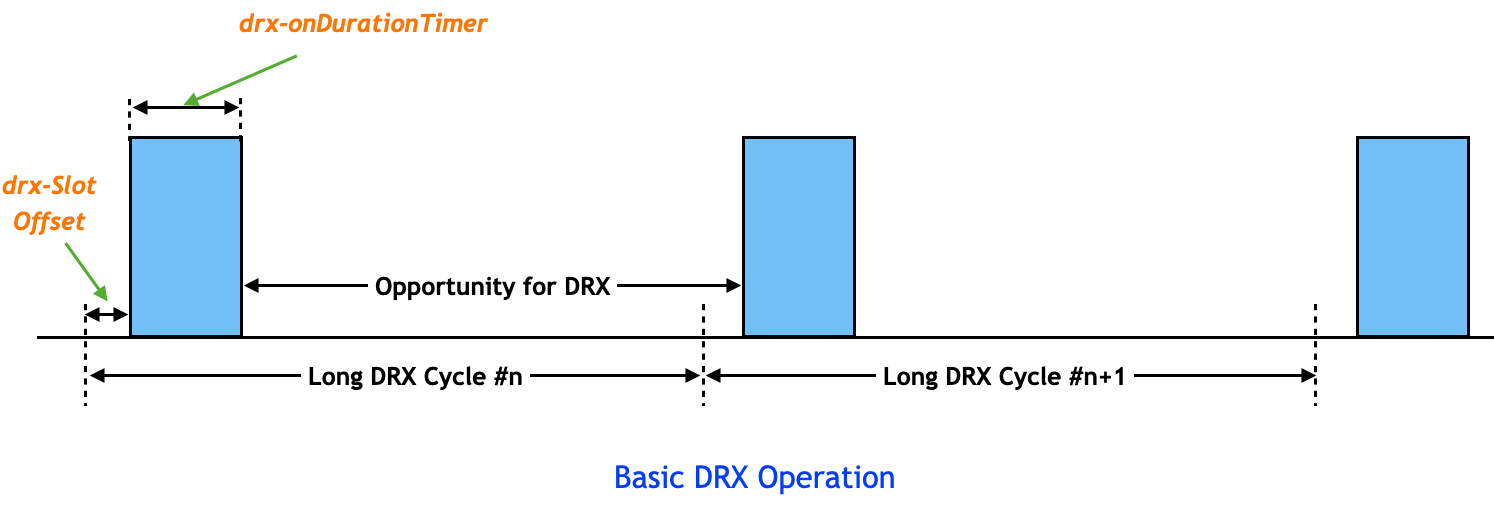
\includegraphics[width=\linewidth]{Pictures/Basic DRX Operation.png}
    \label{fig:basic-drx-operation}
    \caption{Basic DRX Operation}
\end{figure}
    
    \item \textit{drx-onDurationTimer}: a fixed timers at the beginning of every DRX cycle where UE is awake and listening for the control channel. When the timer expires, UE return to sleep if there is no messages on PDCCH as shown on figure \ref{fig:basic-drx-operation}. This timer takes values in multiples of 1/32 ms or in ms (up to 1600 ms).
    \item \textit{drx-InactivityTimer}: a fix timer that starts after a PDCCH occasion which indicates a new UL or DL transmission for the MAC entity. TheUE will continue monitoring PDCCH even after the expiration of  the drx-onDurationTimer. Once the inactivity timer times out, UE return to sleep if there is no messages on PDCCH as shown on figure \ref{fig:5g-drx-InactivityTimer}. This timer takes values in multiples of ms (up to 2560 ms).
\begin{figure}
    \centering
    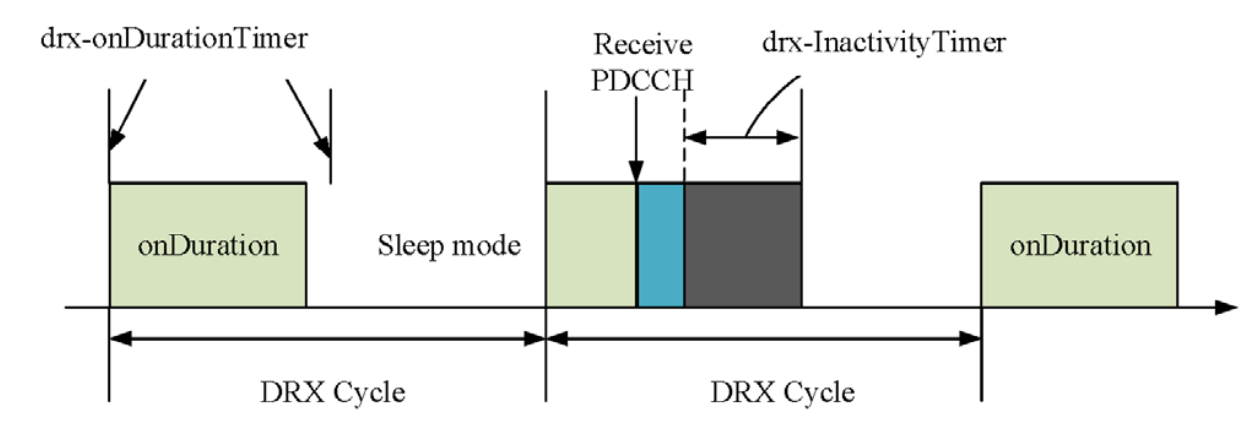
\includegraphics[width=\linewidth]{Pictures/Schematic diagram of drx-InactivityTimer.png}
    \label{fig:5g-drx-InactivityTimer}
    \caption{Schematic diagram of drx-InactivityTimer}
\end{figure}

    \item \textit{drx-ShortCycle}: UE can be configured with shorter DRX cycle by setting this optional parameter. The duration of short DRX cycles can have values in the range between 640 ms.
    
    \item \textit{drx-ShortCycleTimer}: UE switches to operate in long DRX cycles after a number of short cycles with no activity. This number is defined by drx-ShortCycleTimer and has integer values up to 16.
\begin{figure}
    \centering
    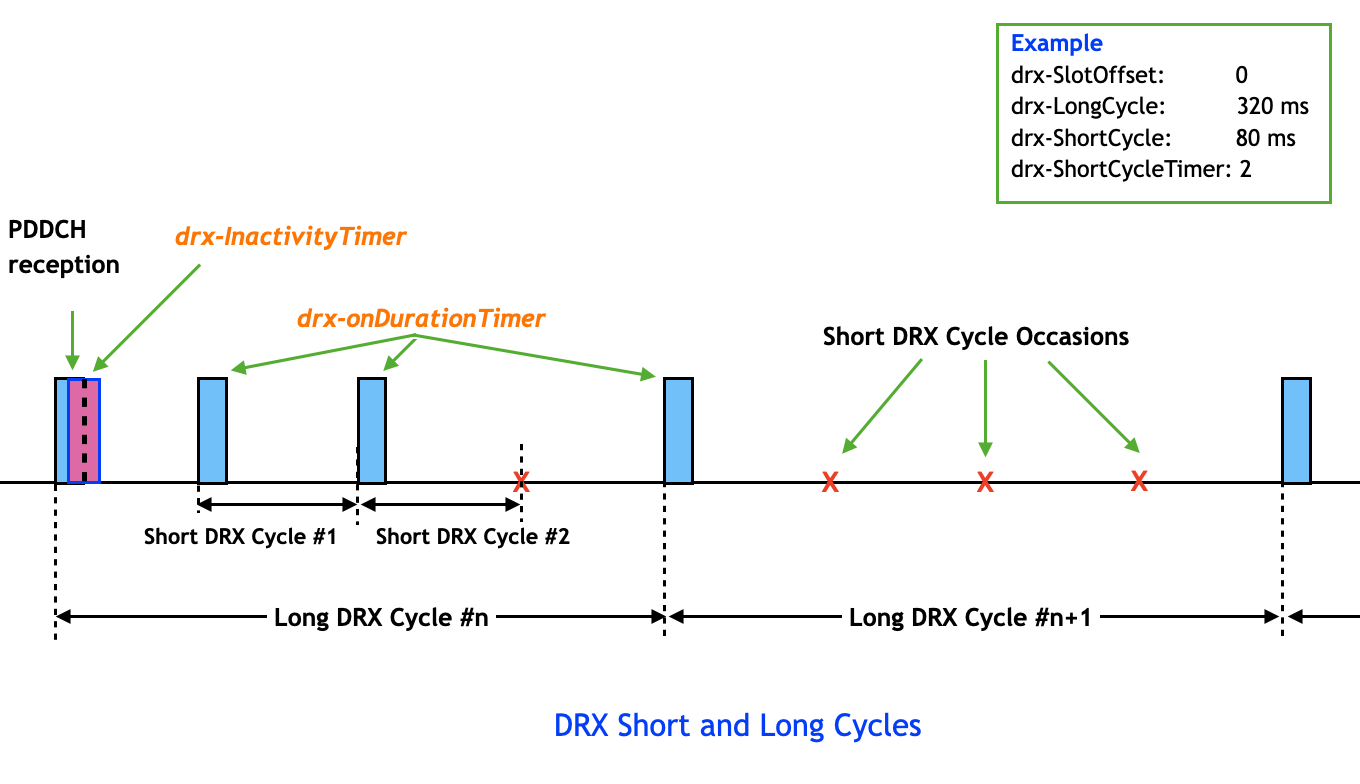
\includegraphics[width=\linewidth]{Pictures/Schematic diagram of drx-ShortCycleTimer.png}
    \label{fig:5g-drx-ShortCycleTimer}
    \caption{Schematic diagram of drx-ShortCycleTimer}
\end{figure}

\end{itemize}

%%%%%   Transition between CDRX and IDRX %%%%%%
A CDRX cycle starts with ON duration period in which UE checks for control messages, i.e., DCI, on PDCCH channel. If UE has detected a packet arrival, it starts the drx-InactivityTimer (This timer is restarted as long as UE still have an ongoing connection). Upon the expiry of the drx-InactivityTimer, UE enters short DRX sleep cycle and subsequently switch to long DRX after several iteration of short cycles as depicted in figure \ref{fig:5g-drx-ShortCycleTimer}. following a configured number of long DRX cycles the network releases UE radio access context and teh UE enters to RRC\_Inactivity and later RRC\_Idle modes where it can benefit from an extended IDRX cycles.



%%%%%   Intro to Paging %%%%%%
UEs in inactive/idle states do not have any active session. However, while sleeping, the UE is required to wake up in a periodic manner to listen to paging messages, and short messages, i.e., System Information (SI) update notifications and emergency notifications (Earthquake/Tsunami Warnings (ETWS), Commercial Mobile Alerts (CMAS)). Paging procedure allows the network to reach UEs in inactive and idle modes. In RRC\_IDLE, the UE receives paging messages initiated by the core network. On the other hand, in RRC\_INACTIVITY, the paging control channel (PCCH) carries RAN-initiated paging. In NR, the same paging/short messages are sent over all beams and it is up to the UE to select the suitable beam by sensing SSB blocks.



%%%%%   How Paging works %%%%%%
Since mobile networks are synchronized communication systems, UE can wake up only at specific time instants, so called, paging occasion (PO). A PO consist of a set of PDCCH monitoring occasions located in the pre-configured pagingSearchSpace as specified in TS 38.213 \cite{3gpp_nr_2022-1_38.213}. Multiple PO(s) form a a Paging Frame (PF) that is equal to one Radio Frame (10 ms). In practice, a PO is transmitted over two parts, PDCCH and an associated PDSCH \cite{esswie_power_2022}. UEs scan the configured PDCCH search space and and search for a paging indication whose CRC is scrambled by P-RNTI. Upon the detection of a paging indication the UE will decode the associated PDSCH looking for the pagingRecordList and to check if it is among the paged UEs.

%%%%%   How UE knows which PF to listen to %%%%%%
The UE monitors one paging occasion (PO) per DRX cycle. UE is able to precisely calculate and determine the System Frame Number (SFN) that carries its PF/PO using the following parameters as specified in Clause 7 in TS 38.304 \cite{3gpp.38.304}:
 \begin{itemize}
     \item T: IDRX cycle of the UE
     \item N: number of total paging frames in T
     \item N$_{s}$: number of paging occasions for a PF
     \item UE\_ID: 5G-S-TMSI stored in USIM
 \end{itemize}

% -   Possible to go in details about the calculation of PF/PO and the concepts of H-SFN, PTW, ...
% -   Adding illustrative figures to differentiate between SFN and H-SFN and how PF/PO occurs in them


%%%%%   Details on the IDRX and the initial eDRX %%%%%%
The value of T (PagingCycle) comes from two different sources. The first is defaultPagingCycle which is broadcasted by the gNB to all UEs through system information messages (SIB1). The second source is UE-specific cycle defined by RRC and/or upper layers. The UE sets the IDRX cycle to the minimum between these two values. PagingCycle is an integer number of radio frames and has a maximum values of rf256 $\approx$2.56 s. This upper bound were later extended and specified in Rel-17 to 10.24 s which corresponds to 1024 radio frame, i.e., the maximum allowed SFN.

%%%%%   Introducing eDRX in RedCap %%%%%%
In RedCap study phase a further extension of IDRX cycle, beyond 10.24 s, were discussed. The main objective was to study the potential power-saving gain and the possible mechanisms to achieve this extension. The proposed approach is to reuse the applicable parts of eDRX mechanism used in LTE RAN, including the usage of Hyper-SFN (H-SFN) and Paging Time Window (PTW) see clause 7.4 in TS 38.304 for more details. This mechanism was originally designed for NB-IoT and LTE-M to allow the to benefit from long eDRX cycles up to few hours. The upper bound of eDRX cycles is limited the upper limit of the H-SFN (1048576 radio frame $\approx$2.91 hrs) and its supported from 5GC (for RRC\_IDLE) since NB-Iot and LTE-M are connected to it.

 %%%%%   What is the performance enhancement?   %%%%%%
The evaluation results submitted by several vendors and summarized in Annex E.1 in TR 38.875 \cite{3gpp.38.875} present a clear power saving enhancement of extending eDRX beyond 10.24s. The results showed a power saving in the range of 80-90$\%$ when using a DRX cycle of 10485.76 s compared to the normal IDRX setting (2.56 s). The study also showed that UEs start to experience a clear power saving gain when eDRX cycle is in the range from 10.24 seconds up to few minutes. This reduction in the energy consumption  may substantially extend the battery lifetime of the UE which is an important requirement for some use cases like industrial wireless sensors.
 
 %%%%%   what is the recommended configuration to be specified in WI   %%%%%%
 Based on the aforementioned advantages, it was decided to in the RedCap work item to specify the support of an extended DRX cycle of 10485.76 s for RedCap devices to be used in both RRC\_IDLE and in RRC\_INACTIVE states. The full details of the mechanisms and feasibility of this extension is still ogoing topic and needs further review with SA2, CT1 and/or RAN4 groups.



\subsection{RRM relaxation for stationary devices}
\label{sec:5-2}


% Main Question this section tries to answer:
%     -   What kind of measurements the UE perform? and why?
%     -   What is the problem of this system of work? (Unnecessary for stationary)
%     -   What is the solution? (RRM measurement relaxation)
%     -   How this solution works? (Triggers and mechanisms)
%     -   What is special in RedCap and what was standardized?

%%%%%   Few words about mobility and RRM meausrements in 5G?   %%%%%%
One of the fundamental characteristics of cellular networks is the support of mobility. Mobility management encapsulates a list of operation, including, measurements, cell selection/(re)selection, and handover. Both gNB and UE cooperate to achieve these RRM-related operations that are done seamlessly to end user. gNB will configure UEs with the required parameters to achieve intra-frequency, inter-frequency cells, and inter-RAT cell selection/re-selection following the requirements specified in TS 38.133 \cite{3gpp.38.133}. The configuration includes defining parameters like the required frequency points, the periodicity and number of measured samples. UEs will report to the gNB the values of reference signal received power (RSRP), reference signal received quality (RSRQ), and Signal-to-Interference-and-Noise Rate (SINR) measured from both the serving and neighbouring cells. Such RRM measurements will guarantee that the UE is camping to the best available cell and ensure a good quality of of communication.
%%%%%   What is the problem ?  %%%%%%

In 5G network, mobility management is a challenging task, especially, with the introduction of new technologies such as Beamforming. This means that to make sure UE is connected to the best available beam it need to perform a precise evaluation of all the possible beams. Even though these measurements are essential to achieve the best performance, they are in some scenarios either unnecessary or not optimized for the mobility profile of the UE. This can lead to excessive power consumption that can drain the UE battery. In some use-case such as industrial wireless sensors and Video Surveillance the UE are more or less stationary and the required RRM measurements can be relaxed.
%%%%%   What is the solution? (RRM measurement relaxation)    %%%%%%
Therefore, already in Rel-16, 3GPP has defined a new power-saving technique to mitigate the aforementioned problem of unnecessary measurements. It was one of the suggested features in study on UE power saving in NR (TR 38.840) \cite{3gpp.38.840}.

%%%%%   What is RRM measurement relaxation?    %%%%%%
 RRM measurements relaxation aimed to specify less frequent UE-specific RRM measurements that adapt the mobility state of the terminal. This feature can be initiated once the UE fulfils some criteria, so called, triggers. RRM Measurement relaxation triggers are configured to the UE by the serving cell through SIB messages. In Rel-16, two triggers were primarily specified: \textit{UE with low mobility} and \textit{UE not at cell edge}. According to TS 38.804, they are defined as followed:\\

 %%%%%   Triggering Criteria    %%%%%%
\subsubsection*{\textbf{Criterion for UE with low mobility}} This trigger defines UEs that are in low mobility state. It based on the fact that the level of RSRP does not dramatically change when UE is not moving fast. UE will monitor the variations in RSRP level received from the serving cell within a duration of $T_{SearchDeltaP}$, This condition can be translated in the following formula:
\begin{equation}
Srxlev_{Ref}-Srxlev<S_{SearchDeltaP}
\label{equ:low-mobility-criterion}
\end{equation}
Where $Srxlev$ and $Sexlev_{Ref}$ are the current and reference Cell selection RX level value (in dB) and these values are directly driven from the measured RSRP level (See clause 5.2.3.2 in TS 38.804). $S_{SearchDeltaP}$ specifies the threshold (in dB) on Srxlev variation. The value of $Sexlev_{Ref}$ is updated with the current level in three conditions: After the selecting or re-selecting a new cell, if the UE is moving toward the center of the cell (i.e., $Srxlev_{Ref}-Srxlev<0$), and finally if the condition in (\ref{equ:low-mobility-criterion}) has not been met for $T_{SearchDeltaP}$. We see that the level of "low mobility" is not strict and is defined by choosing the value of $T_{SearchDeltaP}$ and  $S_{SearchDeltaP}$.\\
\subsubsection*{\textbf{Criterion for UE not at cell edge}} This trigger defines UEs that are located not the edge of the serving cell. It compares the current level of RSRP with a configured threshold $S_{SearchDeltaP}$, communicated to the UE SIB messages:
\begin{equation}
Srxlev>S_{SearchThresholdP}
\label{equ:not-at-the-edge-criterion}
\end{equation}
If the level of the measured RSRP (and subsequently $Srxlev$) is grater than a certain threshold ($S_{SearchThresholdP}$), the UE is considered close to the cell center and less likely to camp to a another neighbour cell. This permits the UE to relax the mobility management setting by having less frequent RRM measurement and save more power.

Due to the stationary property of some of RedCap use cases, new triggers for RRM measurement relaxation can be introduced. RAN2 group, during RedCap study phase TR 38.875 \cite{3gpp.38.875}, has discussed several new triggering enhancement including:
\begin{enumerate}
    \item Introduce of stationary UE state,
    \item Use beam measurements to determine UE mobility state,
    \item Define the mobility property (e.g, Sattionary) of the UE in the subscription information in USIM.
\end{enumerate}

%%%%%   Enhancement in RedCap   %%%%%%
In fact, in the work item \cite{3gpp_revised_2022-1_RP-220966}  of RedCap following the study phase two triggering criteria have been specified for RedCap devices TS 38.804 \cite{3gpp_study_nodate-4_38.804}:
\subsubsection*{\textbf{Criterion for a stationary RedCap UE}} This trigger defines RedCap UEs that are in stationary state. It follows the same approach used in the low mobility criterion by sensing the variation of the level of RSRP measured from the serving cell within a duration of $T_{SearchDeltaP-Stationary}$:
\begin{equation}
Srxlev_{RefStationary}-Srxlev<S_{SearchDeltaP-Stationary}
\label{equ:low-mobility-criterion}
\end{equation}


\subsubsection*{\textbf{Criterion for a stationary RedCap UE not at cell edge}} This trigger combines the two previous criteria and triggers an intensive RRM measurement relaxation once the UE fulfills both "Stationary" and "no at cell edge" conditions. 


%%%%%   What are the methods of RRM relaxation    %%%%%%

Once the UE fulfils any of the aforementioned conditions it can start RRM relaxation operation. Several methods have been discussed during the study phase of RedCap and in previous work items in 3GPP (R2-1912335 \cite{3gpp_ue_2019_R2-1912335}, R2-1912334 \cite{3gpp_rrm_2019_R2-1912334}, and R2-1912531 \cite{1912531_R2-1912531}) on how to achieve RRM relaxation, including:
\begin{enumerate}
    \item Increase the interval between RRM measurement
    \item Reduce the number of neighboring cells to be measured
    \item Reduce the number of measured carrier frequencies
    \item Reduce the number of the monitored reference signals
\end{enumerate}
The methodology that has been adopted so far in the NR standard TS 38.804 \cite{3gpp.38.304} is based on increasing the RRM measurements cycle. This is done by skipping some measurement occasions as illustrated on figure \ref{fig:rrm-relaxation}. UE will have will perform RRM measurements every N DRX cycle where N is a scaling factor that is communicated to UE and takes the values as defined in TS 38.133 \cite{3gpp.38.133}.

\begin{figure}
    \centering
    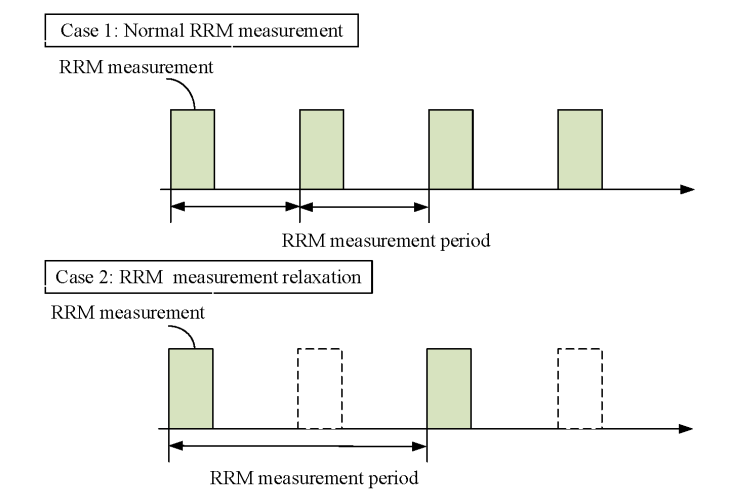
\includegraphics[width=\linewidth]{Pictures/RRM measurement relaxation.png}
    \label{fig:rrm-relaxation}
    \caption{Example of RRM measurement relaxation}
\end{figure}

%%%%%   What are the postive and negative impact?      %%%%%%
Different companies have contributed to the study item of RedCap [] by evaluating and analysing the gain and impact of using RRM measurement relaxation. One source (R2-2100459 \cite{3gpp_tp_2021_R2-2100459} have showed a power-saving gain of $3.6\% - 26.6\%$ when increasing the RRM measurement cycle 4 times with different UE states of idle/inactive and connected modes. This comes at the expense of slight increase in the handover failure rate of $0.26\%$.
Another contribution from Huawie (R2-2009116 \cite{3gpp_further_2020_R2-2009116}) showed an enhancement of $25\%$ in UE power saving by increasing RRM measurement intervals from few seconds to 1 hour. It also showed a $13.54-16.25\%$ power saving gain when relaxing the detection of SSBs block by $62.5-75\%$.
Ericsson on the other hand (R2-2009620) \cite{3gpp_redcap_2020_R2-2009620} claimed that the power saving gained by increasing the measurement intervals beyond one hour (the maximum possible in NR Rel-16) is insignificant. There conclusion was based on the evaluation of UEs that are in RRC\_IDLE or RRC\_INACTIVE states. 

%   Should we put a paragraph to connect the two sections (I do not think so)

\section{RedCap impact on network performance}
\label{sec:6-redcap-impact}
The third main objective of the study item of RedCap was to analyze and evaluate the potential impact and performance degradation arising from the limitation of RedCap devices. The  proposed features, presented in Sections \ref{sec:4-complexity-reduction} and \ref{sec:5-power-saving}, have a great advantages in terms of lowering the device cost/complexity and enhancing the UE battery lifetime. However, an impact on system performance is expected and therefore more detailed (quantitative) evaluation is required to estimate the degradation and enable some functionalities to mitigate or limit it. Two main performance indicators were largely discussed in TR 38.875 \cite{3gpp.38.875}: Coverage Loss and Network Capacity/Spectral-Efficiency. We present in the following subsections the evaluation methodologies agreed on and the final results/takeaway.  

\subsection{Coverage Analysis}
\label{sec:6-1}
% -   What are the potential sources of problem? (Do not forget the small form factor)
% -   What is the metric used to assess the coverage? (MIL, MPL, MCL) (Describe the formula with figure if possible)
% -   What are the used channels/msgs? (PDCCH, PDSCH, ...) 
% -   what are the scenarios parameters?(Urban, Rural, ...)
% -   What are the steps to perform the evaluation? (Two steps: LLS and MIL calc)
% -   What are the results and final take away
% -   What are the proposed coverage recovery techniques?


%%%%%   The potential source of problem     %%%%%%
RedCap devices are expected to experience a coverage loss due to some of the complexity reduction features. The main impact on coverage are coming form the following points:
\begin{itemize}
    \item Reduced number of UE Rx Antenna: This feature will cause a loss in spatial diversity which can affect the quality of received signal and subsequently the coverage 
    \item UE bandwidth Reduction: RedCap device will loose in frequency diversity where it will be limited to operate on a smaller bandwidth. This can lead to a coverage loss in some propagation scenarios.
    \item Antenna efficiency loss: the smaller size of RedCap device in some use-cases such as wearables will affect the antenna gain. The estimated coverage loss is around 3 dB.
\end{itemize}

%%%%%   The metric to estimate the loss     %%%%%%
To analyze the coverage performance, link budget evaluation was used. There exist several formulas used to calculate link budget such as, Maximum Path Loss (MPL), Maximum Coupling Loss (MCL), Maximum Isotropic Loss (MIL). Both MPL and MIL include the antenna gains. However, in consistence with the agreement at study item "TR 38.830 Study on NR coverage enhancements" \cite{3gpp_study_nodate-3_38.830}, it was decided to use MIL. MIL is used to derive the relative differential values between channels and identify the bottlenecks. MIL = Total transmit power – Receiver sensitivity – Tx loss – Rx loss + gNB antenna gain + UE antenna gain. More details on the link budget template can be found in Annex A.3 TR 38.830 \cite{3gpp_study_nodate-3_38.830}. \textcolor{red}{We can add some figure like \ref{fig:MIL-diagram}}

\begin{figure}
    \centering
    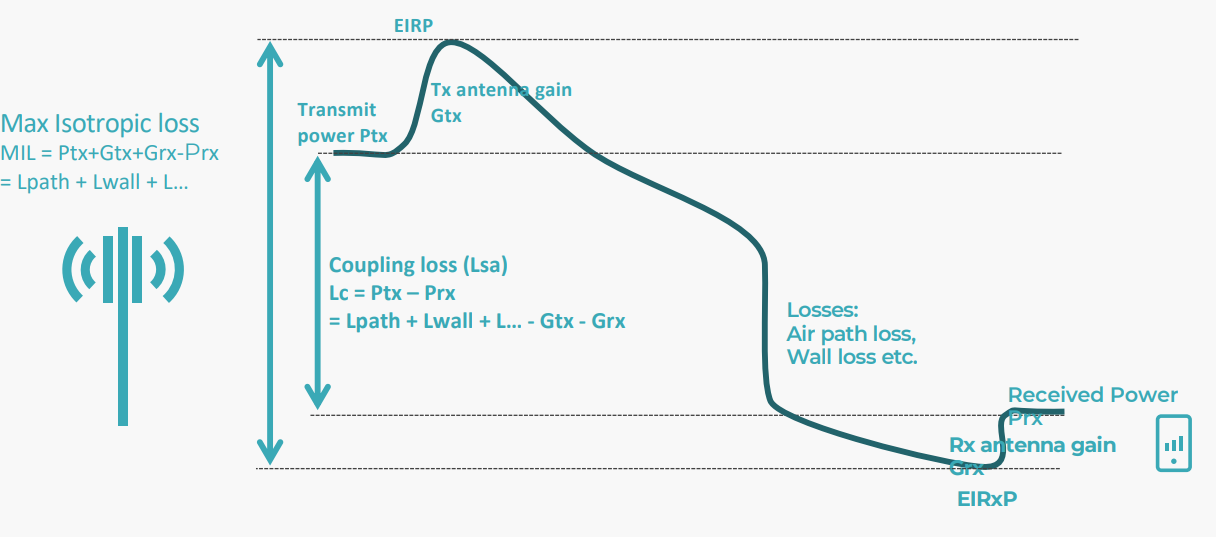
\includegraphics[width=\linewidth]{Pictures/Link budget representation.png}
    \label{fig:MIL-diagram}
    \caption{Representation Maximum link budget}
\end{figure}

%%%%%   The metric to estimate the loss  (MIL)   %%%%%%
Since any of the physical channels can limit the coverage of UE, different types of control and data channels along with the random-access channels where used to carry out the link budget evaluation. A list of the main considered channels and the associated messages are given in table \ref{table:coverage-evaluation-physical-channels}
\begin{table}
\centering
\caption{Physical channels used in coverage evaluation}
\begin{tabular}{| m{0.08\linewidth}  m{0.8\linewidth}|} 
 \hline
    \textbf{Name}  &  \textbf{Description} \\
\hline
    PRACH & Physical Random Access Channel is used by UE to send a preamble in oreder to initiate the connection\\
\hline
    PBCH & Physical Broadcast Channel carries system information messages and the primary and secondary synchronization signals PSS/SSS\\
\hline
    PDCCH & Physical DL Control Channel conveys DCI to UEs e.g., scheduling infromation\\
\hline
    PDSCH &  Physical DL Shared Channel is used to carry UE data on the DL\\
\hline
    PUCCH &  Physical UL Control Channel is used to send feedback to gNB e.g., acknowledgments and channel-state reports\\
\hline
    PUSCH &  Physical UL Shared Channel is used to carry UE data on the UL\\
\hline
    Msg2 &  Message 2 or Random Access Response (RAR) is an indication from the gNB about the reception of UE preamble and carries the uplink grants for Msg.3\\
\hline
    Msg.3 &  Message 3 is used by UE to transmit RRC message(e.g, RrcRequest) and includes information about the device identity and capabilities\\ 
\hline
    Msg4 &  Message 4 or Contention Resolution message confirms that the gNB has correctly identified the UE, and resolved the possible contention and it transfers the UE to RRC\_connected state\\
\hline
\end{tabular}
\label{table:coverage-evaluation-physical-channels}
\end{table}

%%%%%   The Scenario Parameters      %%%%%%
The same coverage evaluation assumptions of the Rel-17 Coverage enhancement SI TR 38.830 were reused in the RedCap Study item. Three propagation scenarios has been studied: Rural and Urban in FR1 and Indoor scenario in FR2. A list of the main parameters of each of these scenarios are summarized in table \ref{table:scenarios-parameters}. Table \ref{table:scenarios-parameters} also includes the common assumptions and the specifications used to differentiate between RedCap and reference NR device.
\begin{table}
\centering
\caption{Physical channels used in coverage evaluation}
\begin{tabular}{|m{0.2\linewidth} | m{0.12\linewidth} |  M{0.15\linewidth}| M{0.15\linewidth} | M{0.15\linewidth}|} 
 \hline
    \multicolumn{2}{|c|}{\textbf{Scenario Parameters}}  & \textbf{Rural}  &  \textbf{Urban} & \textbf{Indoor} \\

\hline
    \multicolumn{2}{|c|}{Carrier frequency} & 0.7 GHz & 2.6 GHz and 4 GHz  & 28 GHz\\
\hline
    \multicolumn{2}{|c|}{Sub-carrier spacing} & 15 kHz & 30 kHz & 60 kHz\\
\hline
    \multicolumn{2}{|c|}{Duplexing} & FDD & \multicolumn{2}{c|}{TDD}\\
\hline
   \multicolumn{2}{|c|}{Delay Spread} &  \multicolumn{2}{c|}{300 ns} & 30 ns\\
\hline
    \multicolumn{2}{|c|}{gNB TX chains} & 2 & 4 & 2\\
\hline
    \multicolumn{2}{|c|}{gNB RX chains} & 2 & 4 & 2\\
\hline
    \multicolumn{2}{|c|}{UE TX chains} & \multicolumn{3}{|c|}{1}\\
\hline

    \multirow{2}{*} {UE RX chains} & Ref. NR & 2  & 4 & 2 \\
    \cline{2-5}
    &   RedCap  &  \multicolumn{3}{|c|}{1 or 2}  \\
\hline
    \multirow{2}{*} {UE bandwidth} & Ref. NR & 20 MHz & \multicolumn{2}{|c|}{100 MHz} \\
    \cline{2-5}
    &   RedCap  &  \multicolumn{2}{|c|}{20 MHz} & 50 MHz or 100 MHz  \\
\hline
    \multicolumn{2}{|c|}{UE speed profile} & \multicolumn{3}{|c|}{3 km/h}\\
\hline
    \multicolumn{2}{|c|}{UE antenna correlation} & \multicolumn{3}{|c|}{low}\\
\hline
\end{tabular}
\label{table:scenarios-parameters}
\end{table}

%%%%%    What are the steps to perform the coverage evaluation?  %%%%%%
For both RedCap and reference UEs, the target performance requirements of each of the aforementioned physical channels/signals is defined, i.e., min throughput, block error rate (BLER), no. of HARQ re-transmission, etc. After that, the coverage evaluation to determine if RedCap device requires coverage recovery is carried out following three main steps:
\begin{enumerate}
    \item  Perform a Link-level Simulation (LLS)  to figure out the required SNIR that meet the performance target of each of the examined physical channels. The simulation are done with respect to the parameters defined in table \ref{table:scenarios-parameters}.
    \item Use the results of the LLS (i.e., SINR levels) to calculate the link budgets MILs.
    \item Once the MIL levels of all different channels are calculated, the amount of required coverage recovery is identified by the link budget (MLI) of the bottleneck channel for the reference NR device within the same deployment scenario (option 3). The bottleneck channel is the physical channel that have the lowest MIL.
\end{enumerate}
In Summary, a RedCap UE that has physical channels who experiences a MIL worse than the bottleneck channel of a reference NR device in the same propagation scenarios needs to compensate the difference.  

%%%%%    Summary of the results of coverage evaluation  %%%%%%
Different companies have contributed to RedCap study by performing the link budget analysis. The results of the simulation of different sourcing companies can be found in Annex C of TR 38.875 \cite{3gpp.38.875} and in R1-2009293 \cite{3gpp.R1-2009293}. As a conclusion of coverage evaluation of RedCap devices the following outcomes are made:
\begin{itemize}
    \item In FR1, for both Rural and Urban scenarios, due to the size limitation of RedCap device a reduced antenna efficiency of 3 dB are estimated. As a result, both PUSCH and Msg3 experience a MIL level that is less than the the bottleneck channel of the reference NR UE and a coverage recovery is needed. However, the other UL physical channels do not require a coverage compensation since they have a MIL level higher than the bottleneck channel. For the DL physical channels, the coverage is dependent of the frequency bands (i.e., 0.7 GHz, 2.4 GHz, or 4 GHz) and the assumptions of the DL Power Spectral Density (DL PSD). The most affected signals are Msg2 and Msg4 with a potential degradation of 6 dB, especially, for RedCap UEs with 1 Rx. This coverage degradation can be mitigated by using the existing  Transport Block Size (TBS) scaling technique
    \item In FR2, the problem of RedCap device size and the reduced antenna efficiency is less efficient since at mm Waves the antennas have small size.  Therefore, the the MIL levels of UL channels are equivalent to the ones of the reference NR UE and no coverage recovery is needed on the UL. On the other hand for the DL channels, a coverage recovery in the range [2-3 dB] is needed for PDSCH, for RedCap UE with 50MHz BW and 1Rx.
\end{itemize}

%%%%%    Coverage recovery techniques  %%%%%%

Regarding the coverage recovery, no new solutions were specified for RedCap UEs as a result of the work item.  However, RedCap devices are assumed to reuse the existing Uplink coverage enhancement solutions (e.g., PUSCH repetition)  specified in the Rel-17 NR Coverage Enhancement WI (NR\_cov\_enh) TR 38.830\cite{3gpp_study_nodate-3_38.830}. Other techniques form Rel-15/16 (e.g., TBS scaling) are also available for RedCap UEs.






\subsection{Capacity Analysis}
\label{sec:6-2}

%%%%%    The source of problem of capacity  %%%%%%
Similar to the coverage performance, the introduced complexity reduction features of RedCap devices are expected to negatively affect the overall system capacity. Simplification like, reducing the number of antennas and the modulation order have a direct impact on the spectral efficiency and consequently the system capacity. Therefore, a quantitative evaluation of this impact has to done before approve these features.

%%%%%    The agreed simulation assumptions  %%%%%%
A system-level simulations must be conducted to evaluate the system performance. It was agreed to re-use the simulation assumptions from TR 38.802 \cite{3gpp_study_nodate-2_38.802} as a baseline. Some additional modifications were proposed for the study case of RedCap. A list of the main simulation parameters for both the RedCap and Reference NR devices are given in Table \ref{table:sls-assumption}. The rest of simulation parameters can be found in Table 6.4-1 and Table D-1 in TR 38.875 \cite{3gpp.38.875}. Several traffic models were used, including full buffer traffic and burst traffic such as File Transfer Protocol model 3 (FTP3) and Instance Messaging (IM) where each of these models characterized by different packet size and inter-arrival time. The overall Resource Utilization (RU) in the cell is connected to number of the UEs and the traffic model used. The complexity reduction features of RedCap devices are consistent with one presented in Section \ref{sec:4-complexity-reduction}. The metric used to evaluate the system performance is the average spectral efficiency (SE) and it is defined as follows:
\begin{equation}
\textrm{SE}=\frac{\textrm{cell average throughput (Mbps)}}{\textrm{cell bandwidth (MHz)}\times\textrm{RU}}
\label{equ:spectral-efficiency}
\end{equation}


\begin{table}
\centering
\caption{Assumptions for SLSs}
\begin{tabular}{|p{0.23\linewidth}| p{0.33\linewidth} |  p{0.33\linewidth}|} 
 \hline
    \textbf{Parameters}  & \textbf{RedCap UE}  &  \textbf{Reference UE}\\
\hline

\begin{itemize}[leftmargin=0,label={}]
        \item Scenarios
    \end{itemize}  & 
    \multicolumn{2}{|p{0.66\linewidth}|}{
    \begin{itemize}[leftmargin=*]
        \item Dense Urban: 2.6 GHz and 4 GHz (TDD)
        \item Indoor: 28 GHz (TDD)
    \end{itemize} 
    }\\
\hline

    \begin{itemize}[leftmargin=0,label={}]
        \item Traffic Model
    \end{itemize}  & 
    \begin{itemize}[leftmargin=*]
        \item Full buffer (optional)
        \item FTP model 3
        \item IM traffic model
    \end{itemize}   &

    \begin{itemize}[leftmargin=*]
        \item Full buffer (optional)
        \item FTP model 3
    \end{itemize}   \\

\hline
    \begin{itemize}[leftmargin=0,label={}]
        \item Traffic load
    \end{itemize}  & 
    \multicolumn{2}{|p{0.66\linewidth}|}{
    \begin{itemize}[leftmargin=*]
        \item Full buffer (optional): 10 users per cell
        \item Other traffic models: low ($<30\%$) and medium ($30-50\%$) resource utilization
    \end{itemize} 
    }\\
\hline
    \begin{itemize}[leftmargin=0,label={}]
        \item Scheduled BW
    \end{itemize}   & 
    \begin{itemize}[leftmargin=*]
        \item 20 MHz in FR1
        \item 50 or100 MHz in FR2
    \end{itemize}   &
    
    \begin{itemize}[leftmargin=*]
        \item 100 MHz for FR1/FR2
        
    \end{itemize}   \\
\hline
    \begin{itemize}[leftmargin=0,label={}]
        \item Max modulation order
    \end{itemize}  & 
    \begin{itemize}[leftmargin=*]
        \item 64QAM for DL
        \item 16QAM for UL
    \end{itemize}   &
    
    \begin{itemize}[leftmargin=*]
        \item 254QAM for DL
        \item 64QAM for UL
    \end{itemize}   \\
\hline

    \begin{itemize}[leftmargin=0,label={}]
        \item UE Rx / MIMO layers
    \end{itemize}  & 
    \begin{itemize}[leftmargin=*]
        \item 1Rx or 2Rx
    \end{itemize}   &
    
    \begin{itemize}[leftmargin=*]
        \item 4Rx in FR1
        \item 2Rx in FR2
    \end{itemize}   \\
\hline
    \begin{itemize}[leftmargin=0,label={}]
        \item  RedCap UE ratios
    \end{itemize}  &  
    \multicolumn{2}{|p{0.66\linewidth}|}{
    \begin{itemize}[leftmargin=*]
        \item $0\%,\: 25 \%,\: 50 \%,$ or $100 \%$ of the UEs in the cell are RedCap devices
    \end{itemize} 
    }  \\
\hline

\end{tabular}
\label{table:sls-assumption}
\end{table}

%%%%%    The agreed SLS results  %%%%%%
The results of the SLS from different companies are gathered in the Tables D-1 to D-25 in Annex D of TR 38.875 \cite{3gpp.38.875}. The evaluations covers different combinations of the parameters presented in Table \ref{table:sls-assumption}. The outcome of the capacity and spectral efficiency evaluation can be summarized in the following:

\begin{itemize}
    \item In the case where both types of UEs have a burst traffic, FTP model 3 is assumed for eMBB users and IM traffic for RedCap devices. The results shows that introducing RedCap devices will have a marginal impact on the user throughput of other eMBB UEs and the overall system capacity. It worth noting that given the considered traffic models, the RedCap devices generates 0.1 MB payload every 2 s (400 kbps) while eMBB devices have 0.5 MB payload every 200 ms (20 Mbps). This means that the generated load of RedCap devices is very limited even in the case high ratio of RedCap devices in the cell. The IM traffic model is only valid for the use cases of video surveillance and industrial wireless sensors where the exchanged traffic is dominated by the UL.
    \item In the case where both devices has a burst traffic of the model FTP3. This evaluation is applicable in the case where RedCap devices are wearables and has more traffic on the DL. The results varies between the sourcing companies. On one hand, Nokia stated that the throughput of eMBB device is not affected by the introduction of RedCap device. On the other hand, Huawei/HiSilicon claimed that the spectral efficiency degradation can reach 30\% and 50\% in the case of having RedCap devices with 1Rx and 2Rx respectively.
    \item Similar conflicted results between companies have been reported in the case when both eMBB UEs and RedCap devices is modeled with a full buffer traffic. Nokia claims a minor degradation in the spectral efficiency while Huawei/HiSilicon showed that the impact can reach 54-70\% depending on the number of Rx chains used for RedCap devices.
\end{itemize}





\subsection{Other Compatibility Concerns}
\subsubsection{Definition and constraining of reduced capabilities}
\subsubsection{UE identification and access restrictions}


\section{Beyond RedCap Rel-17}
\label{sec:7}

% -   Present the work based on Rel-17 RedCap (Saffi "UL enhancement" and Nokia "RRM relaxation" and The )
% -   Present the work of Rel-18 WI (NR\_redcap\_enh), including:
%     -   Justification
%     -   Objective
%     -   Proposed features
%     -   Evaluation
% -   Present the other Rel-18 RedCap WI (NR\_REDCAP\_Ph2), icluding:
%     -   Objective
%     -   It started in Dec 2022, so the study document is not ready yet


%%%%%    Some intro  %%%%%%
At the end of the study phase of Rel-17 RedCap in March 2021, 3GPP published a full technical report TR 38.875 \cite{3gpp.38.875}. It summarizes the overall justification and the objective of this new technology, entitled, RedCap. It also includes a description of all of the proposed features to reduce UE cost/complexity and enhance the power-saving. After this,  several works in academia tried to further investigate the proposed solutions and test its applicability in the frame of 5G system.

%%%%%    Saafi work on UL enhancemant  %%%%%%
Given the coverage loss reported on the UL, especially, PUSCH channel, \cite{saafi_enhancing_2022} highlighted that such degradation might a huge impact on certain categories of RedCap devices. Services like healthcare monitoring and work safety require a reliable real-time UL transmission. Several available 5G techniques to enhance UL performance were discussed, including, Dual Connectivity (DC), Carrier Aggregation (CA) and Supplementary Up Link (SUL). DC and CA were excluded since they both violate the RedCap complexity reduction recommendation of supporting single connectivity mode with operation in a single band at a time. SUL on the other hand can be implemented such that the UE operates at a single frequency band at a time and switches to another the quality of the received signal drops (e.g., from 3.5 GHz band to 700 MHz band). The evaluation of this technique was done through link-level simulations. The results showed an gain in the link budget of 8.33 dB which was reflected in improving the probability of detection and BLER (\textcolor{red}{I found inconsistency in the comparison of using two different preamble sequence for the two bands}). However, this gain in terms of coverage comes at the expense of losing some of the UE throughput and an additional delay due to the switching cost.

%%%%%    Nokia work on RRM Relaxation  %%%%%%
Another work conducted by Nokia team \cite{tayyab_rrm_2021} investigated some modifications on the proposed RRM measurement relaxation feature. It aims to quantify and analyze the power-saving gain while using different thresholds of "cell edge" criterion. The study was done for RedCap UEs with two mobility profiles: Stationary and Pedestrian (3 km/h). For stationary UE, The results showed that reducing the threshold of "Cell edge" can significantly improve UE energy consumption (up to 96\% better than the baseline "No RRM relaxation" case) and without any additional impact in terms of handover failures ratio (HOFR). The pedestrian UEs on the other hand, experienced a substantial increase in the HOFR while reducing the "cell edge" which affected the service continuity.

%%%%%    The work of China on enhanced Paging  %%%%%%
A parallel work on UE power-saving for RedCap devices was provided by \cite{li_radio_2022}. The paper reviewed the existing power-saving techniques in 5G NR. This includes discontinuous reception (DRX), wake-up signal (WUS), RRM relaxation, and Paging enhancement.  The study proposed an approach to enhance the paging for RedCap UEs that are geographically located close to each other. This technique is similar to Paging Sub-grouping specified in Rel-16 (See section 7.3 in TS 38.804 \cite{3gpp_study_nodate-4_38.804}). However, this work was not supported by simulations results that validate the power-saving gain.   

%%%%%    RedCap Rel-18  %%%%%%
\subsection{RedCap in Rel-18}
5G has always aimed to support the industrial automation and digitalization movement and facilitate the transition toward the world of smart cities. In this regard, 5G NR should provide the support for low-tier device segment that fall between the existing LPWA UEs (supported by NB-IoT and LTE-M) and the Rel-17 RedCap devices. Basing on the foundations put in Rel-17 RedCap WI, 3GPP continued in Rel-18 the work on enhanced support of reduced capability NR devices in the work item (NR\_redcap\_enh) \cite{3gpp_revised_2022_RP-223544} RP-223544.

The main objective of the work on Rel-18 RedCap is to expand the 5G market with use cases that have relatively lower cost/complexity and lower power consumption. Following the same logic used in Rel-17, a further reduction of the Bandwidth to 5 MHz is suggested to cut the device cost/complexity. Another simplification regarding the restriction of the UE peak data rate to 10 Mbps was discussed. The proposed features and the analysis of their impact is documented in the technical report TR 38.865 \cite{3gpp_study_2022_38.865}. This extension of RedCap Rel-18 aims to enlarge the range of RedCap application with use cases that need relatively lower cost/complexity, more power-saving devices. However, it is important to note that this expansion is not meant to overlap with the existing LPWA applications.

Another work item related to RedCap has later started in December 2022 entitled "5GS support of NR RedCap UE with long eDRX for RRC\_INACTIVE State" (NR\_REDCAP\_Ph2, SP-220803 \cite{3gpp_5gs_2022_SP-220803}). This work aims to specify the required mechanism to support the . In RRC\_idle state, the 5G system is equipped with the mechanisms required to support a paging cycles beyond 10.24s since it supports both NB-IoT and LTE-M. However, for the RRC\_inactivity state the handling of UE  data/signals is not defined when the UE is unreachable for period more than 10.24s.




\section{Summary of the Study (RedCap)}
\label{sec:7}


A table containing our recommendation for users. This includes how to choose the suitable technology 

A table summarizing our contribution: In one direction RedCap types (Use Cases) and in the other direction the proposed features and we match between them.
\cite{noauthor_5g_2020}

\section{Conclusion}
\label{sec:7-3}

This is new reference \cite{3gpp_study_2021_38.875}\\
This is a link to Section \ref{sec:1-Inro}

\bibliographystyle{IEEEtran}
\bibliography{references}

\end{document}
